% \documentclass[a4paper,10pt]{article} % or whatever
% \documentclass[letterpaper,10pt]{article} % or whatever
\documentclass{article}

% if you need to pass options to natbib, use, e.g.:
     \PassOptionsToPackage{numbers, compress}{natbib}
% before loading neurips_2020

% ready for submission
% \usepackage{neurips_2021}

% to compile a preprint version, e.g., for submission to arXiv, add add the
% [preprint] option:
% \usepackage[final]{neurips_2021}

% to compile a camera-ready version, add the [final] option, e.g.:

% \usepackage[final]{neurips_2020}
\usepackage[preprint]{neurips_2021}
% \usepackage[preprint]{neurips_2021}


% to compile a camera-ready version, add the [final] option, e.g.:


% \newtheorem*{notice}{Notice}

% \theoremstyle{definition}
% \newtheorem{dfn}[equation]{Definition}
% \newtheorem{bigrem}[equation]{Remark}
% \newtheorem{num}[equation]{} % a bit strange, but I do use it!
% \newtheorem{exmp}[equation]{Example}


\newcommand{\ignore}[1]{}
% to avoid loading the natbib package, add option nonatbib:
\usepackage{dsfont}
\input{preamble}
\usepackage{tikz}
\usetikzlibrary{shapes.geometric, arrows}
%  \usepackage{subfigure} 
\pdfminorversion=7

%\floatname{algorithm}{Procedure}
\renewcommand{\algorithmicrequire}{\textbf{Input:}}
\renewcommand{\algorithmicensure}{\textbf{Output:}}
\newcommand{\TV}[1]{\norm{#1}_{\textnormal{TV}}}
\newcommand{\one}[1]{\norm{#1}_{1}}
\newcommand{\bfs}[1]{\textbf{({#1})}}
\newcommand{\typss}{\mathcal{P}_n}

\usepackage[utf8]{inputenc} % allow utf-8 input
\usepackage{microtype}      % microtypography

%\tikzstyle{input} = [rectangle, rounded corners, minimum width=1cm, minimum height=1cm,text centered, draw=black]
%\tikzstyle{process} = [rectangle, minimum width=3cm, minimum height=1cm, text centered, draw=black]
%\tikzstyle{output} = [rectangle, rounded corners, minimum width=1cm, minimum height=1cm,text centered, draw=black]
\title{Information Theory, Statistics and Inequality}
% \author{%
%   Qiyu~Kang, and Wee~Peng~Tay
%  \thanks{First two authors contributed equally to this work.} 
%   \\
%   School of Electrical and Electronic Engineering\\
%   Nanyang Technological University\\
%   Singapore \\
% %   \texttt{songy@ntu.edu.sg, kang0080@e.ntu.edu.sg, wptay@ntu.edu.sg, qding001@e.ntu.edu.sg} \\
%   % examples of more authors
%   % \And
%   % Coauthor \\
%   % Affiliation \\
%   % Address \\
%   % \texttt{email} \\
% }



\begin{document}

\maketitle

\section{A short introdution}
This note is mainly from \cite{cover1999elements}. We use the method of types to calculate the probability of \tb{rare} events and to show the existence of universal source codes.  Note method of types introduced here mainly focuses on \tb{exponents} $a$, either positive or negative, in $e^{na}$,  in an asymptotic way. Proofs are either sketched or skipped with the principle of whether the theorems are obvious and intuitively clear. It is better to view this tutorial together with ``“Inequality and Approximate'' tutorial, especially with the powerful tool Stirling’s approximation in mind since many binomial coefficients, e.g. \cref{method:rem3}, has been better analyzed there.

We first establish the fundamental method of types theory in \cref{sec:method}, which deals with sequences that have the same empirical distribution. Before we proceed to the application of method of types, we introduce the total variation, Kullback-Leibler (KL) divergence  and $\calL_1$ distance, which can be used as a measurement of measure difference \cref{sec:tv}. We then consider the following problems as applications of method of types:
\begin{enumerate}
\item Convergence (a.s.) of Empirical Measure and Weak LLN: We definite two kinds of typical sets $T_{Q}^{\epsilon}$ and $A_{\epsilon}^{*(n)}$, which both have high probability, and show their relations. We show the convergence under KL divergence a.s. and its implication of Glivenko-Cantelli Theorem.  
\item Universal source coding \blue{a reminder: please talk about the error exponent in maximum likelihood decoding for channel and the old paper}
\item  Large Deviation Theory: We give Sanov's Theorem and  Cram\'{e}r-Chernoff Theorem. We show that $Q^n(E)$ essentially determined by $D\left(P^{*}|| Q\right)$, the distance of the \tb{closest} element of $E$ to $Q$. 
\item Conditional probability and limit theorems: We show that given that we are in set $E$, the type $P_{X^n}$ is very likely to be close to $P^{*}$. The main idea is $P^*$ is the dominant term in $E$, given $E$, $P_{X^n}$ observed is close to $P^*$. 
\item Hypothesis Testing
\item Estimation, Fisher Information and the Cram\'{e}r Inequality
\end{enumerate}

\blue{lesson7\_h is also needed, maybe in a separate file talking about entropy, channel, .etc.}
\section{Method of Types}\label{sec:method}
The method of types  deals with sequences that have the \emph{same} empirical distribution.  We derive strong bounds on the number of sequences with a particular empirical distribution and the probability of each sequence in this set. 

\tb{Notations:}

Let $X_{1}, X_{2}, \ldots, X_{n}$ be a random sequence of $n$ symbols from an \emph{alphabet} $\cal{X} =$ $\left\{a_{1}, a_{2}, \ldots, a_{|\cal{X}|}\right\} .$ Except in \cref{ssect:ld_cramer}, we only consider discrete finite alphabet. We use the notation $x^{n}$ and $\bx$ interchangeably to denote a particular sequence sample $x_{1}, x_{2}, \ldots, x_{n}$. $Q^n(\bx) \coloneqq \P{Q^n}(X^n = \bx) = Q(X_1 = x_1)\cdot Q(X_2 = x_2)\ldots \cdot Q(X_n = x_n)$ with the same probability distribution $Q$ for each $X_i$, i.e. $Q^n$ is the product distribution for \gls{iid} $X_i$s. With a slight abuse of notation, $Q^{n}(E)\coloneqq Q^{n}\left(E \cap \typss\right)=\sum_{ \bx : P_{ \bx } \in E \cap \typss} Q^{n}( \bx )$ for any set $E$, where $\typss$ is defined in \cref{method:defP}. We sometimes use notation $\P$ to briefly represent  ``the probability of something'' without specifically saying w.r.t to which distribution and $\P{Q^n}$ to  briefly represent ``the probability of something w.r.t to distribution ${Q^n}$''.


\begin{defa}{\tb{(Type)}}
The type $P_{ \bx }$ (or empirical probability distribution) of a sequence $x_{1}, x_{2}, \ldots, x_{n}$ is the relative proportion of occurrences of each symbol $a\in \cal{X}$:
\begin{align*}
    P_{\bx }(a)= \frac{N(a \mid \bx )}{n} = \frac{1}{n} \sum_{i=1}^{n} 1_{a}\left(x_{i}\right), \forall a \in \cal{X},
\end{align*}
where $N(a \mid \bx )$ is the number of times the symbol $a$ occurs in the sequence $\bx \in X ^{n}$
\end{defa}

\begin{defa}{\tb{(Probability Simplex)}}
The probability simplex $\Delta_m$ in $\Real ^{m}$ is the set of points $z=\left(z_{1}, z_{2}, \ldots, z_{m}\right) \in \Real ^{m}$ such that $z_{i} \geq 0, \sum_{i=1}^{m} z_{i}=1$.
\end{defa}

\begin{defa}{\tb{(Set of All Types)}}\label{method:defP}
Let $\mathcal{P}_{n}$ denote the set of types with denominator  (length) $n$.
\end{defa}

For example, if $X =\{0,1\}$, the set of possible types with denominator $n$ is
\begin{align*}
\typss=\left\{(P(0), P(1)):\left(\frac{0}{n}, \frac{n}{n}\right),\left(\frac{1}{n}, \frac{n-1}{n}\right), \ldots,\left(\frac{n}{n}, \frac{0}{n}\right)\right\}
\end{align*}

\begin{defa}{\tb{(Type Class)}}
The set of sequences of length $n$ with type $P\in \typss$  is called the type class of $P$, denoted $T(P)$ :
\begin{align*}
T(P)=\left\{ \bx \in \calX ^{n}: P_{ \bx }=P\right\}
\end{align*}
\end{defa}

\begin{rema}
$\typss\subseteq \Delta_{|\calX|}$ with dimension $\Delta_{|\calX|}-1$.
\end{rema}

\begin{thma} {\tb{(Size of  $\mathcal{P}_{n}$)}}\label{method:thm1}
There are only a \tb{polynomial} number of types of length $n$.
\begin{align*}
\left| \typss\right| \leq(n+1)^{| \calX |}
\end{align*}
\end{thma}

\begin{rema}\label{method:rem1}
The number of possible sequences is exponential in $n$, it follows that at least one type has \tb{exponentially many} sequences in its type class. 
In fact, the largest type class (w.r.t to size) has essentially the same number of elements as the entire set of sequences, \tb{to first order (of $\log |\calX|$) in the exponent}. See the following remark and \cref{method:thm3}



% : 2^{nlog|X|} (from 11.1.3 with the uniform distribution of the alphabet)
%  2^(-nH(P)) P is the distribution of the alphabet

\end{rema}

\begin{rema}{(type class with largest \tb{size} vs.  type class with largest \tb{probability})}\label{method:rem2}
For of all, they are different. The total number of possible sequences  with length $n$ is $|\calX|^n= 2^{n\log |\calX|}$. By assigning the uniform distribution $U$ to $X_i$, and assume \gls{iid}, we have $T(U)$ is the type class with largest \tb{size}. This is because under the uniform distribution $U$, the size of $T(P)$ is proportional to the probability of $T(P)$ (with rate $1/|\calX|^n$) and $U^n(T(U))\ge U^n(T(P))$ for all $P\in \calP_n$.  (See also \href{https://djalil.chafai.net/blog/2015/08/29/about-the-central-multinomial-coefficient/}{maximality of central multinomial coefficient}). 
From \cref{method:thm3}, we have $|T(U)|\doteq 2^{nH(U)} = 2^{n\log |\calX|}$. (Above explanation for the type class with largest \tb{size} is written for more thinking because the special coincidence of size and probability. Actually we can directly get $|T(U)|$ is the largest from \cref{method:thm3} because $H(U)$ is the largest first order in the exponent.)
In contrast, if $X_i$ s have the distribution $Q$, which is different from $U$ in general, independently and identically, we have $T(Q)$ is the type class with largest \tb{probability} (see \cref{method:lem1}, \cref{method:thm4} and \cref{ld:thm1}). 

\end{rema}

\begin{thma}{\tb{(Probability of A Sequence Sample $\bx$)}}\label{method:thm2}
If $X_{1}, X_{2}, \ldots, X_{n}$ are drawn \gls{iid} according to $Q(\bx)$, the probability of $\bx$ depends only on its type and is given by
\begin{align}
Q^{n}( \bx )=2^{-n\left(H\left(P_{ \bx }\right)+D\left(P_{ \bx }|| Q\right)\right)}
\end{align}
\end{thma} 
\begin{rema}{\bfs{$\P(\text{sample } \bx)$ vs. $\P(\text{type class } T(P))$ vs. $\P(\text{set of type classes } E)$}}\label{method:rem4}
 
 Note in \cref{method:thm2}, it is a particular sequence sample $\bx$, not a type class $T(P)$. Also we have $$Q^{n}( \bx\mid \bx\in T(P) ) =\ofrac{|T(P)|}.$$
 \begin{enumerate}
     \item  \cref{method:thm2} tells us $\P(\text{sample } \bx)$.
     \item \begin{align}
    Q^{n}(T(P_{\bx})) \coloneqq Q^{n}(\bx\in T(P))=|T(P)|2^{-n\left(H\left(P_{ \bx }\right)+D\left(P_{ \bx }|| Q\right)\right)}. \label{method:eq1}
    \end{align}
    To get the asymptotic order of $Q^{n}(T(P))$, see \cref{method:thm4} where the asymptotic order of $T(P)$ is used from \cref{method:thm3}.
    \item \cref{ld:thm1} and \cref{ld:rem1} tell us $\P(\text{set of type classes } E)$ for \tb{nontypical} set $E$.
 \end{enumerate}

\end{rema}

\begin{proof}
\begin{align*}
\begin{aligned}
Q^{n}( \bx ) &=\prod_{i=1}^{n} Q\left(x_{i}\right) \\
&=\prod_{a \in X } Q(a)^{N(a \mid \bx )} \\
&=\prod_{a \in X } Q(a)^{n P_{ \bx }(a)} \\
&=\prod_{a \in X } 2^{n P_{ \bx }(a) \log Q(a)} \\
&=\prod_{a \in X } 2^{n\left(P_{ \bx }(a) \log Q(a)-P_{ \bx }(a) \log P_{ \bx }(a)+P_{ \bx }(a) \log P_{ \bx }(a)\right)} \\
&=2^{n \sum_{a \in X }\left(-P_{ \bx }(a) \log \frac{P_{\bx}(a)}{Q(a)}+P_{ \bx }(a) \log P_{ \bx }(a)\right)} \\
&=2^{n\left(-D\left(P_{ \bx } \| Q\right)-H\left(P_{ \bx }\right)\right)} .
\end{aligned}
\end{align*}
\end{proof}
\begin{cora}
If $\bx$ is in the type class of $Q$, then
\begin{align*}
Q^{n}( \bx )=2^{-n H(Q)}
\end{align*}
\end{cora}




\begin{thma}{\bf{(Size of A Type Class $T(P))$)}}\label{method:thm3}
For any type $P \in \typss$,
\begin{align*}
\frac{1}{(n+1)^{| \calX |}} 2^{n H(P)} \leq|T(P)| \leq 2^{n H(P)}
\end{align*}
\end{thma} 

\begin{rema}{\tb{(subexponential vs. exponential)}}
The restriction of getting an asymptotic order $\binom{n}{k}$ from \cref{method:thm3}: The problem can be viewed as the size of $T(P)$ with type $P=\frac{k}{n}$, and $|\calX|=2$. If $k=o(n)$, type $P=(0,1)$ in the limit, then the bound fails, that means the $k$ need to be a \tb{linear} order of $n$, i.e. $k=O(n)$. In other words, \cref{method:thm3} only works for \textbf{exponential} case with $k=O(n)$. For  \textbf{sub-exponential} case see ``Inequality and Approximate''.
\end{rema}

\begin{rema}{\tb{(first order in the exponent for $|T(P)|$)}}
From \cref{method:thm3}, we know $|T(P)|\doteq 2^{nH(P)}$. See also \cref{method:rem1,method:rem2} for discussions of the largest size of type class.
\end{rema}

\begin{rema}{\tb{(speical case: binary alphabet $|\calX|=2$ )}}\label{method:rem3}
From \cref{method:thm3}, we know 
\begin{align*}
\frac{1}{(n+1)^2} 2^{n H\left(\frac{k}{n}\right)} \leq\left(\begin{array}{l}
n \\
k
\end{array}\right) \leq 2^{n H\left(\frac{k}{n}\right)},
\end{align*}
where the lower bound can be slightly improved to $\frac{1}{n+1} 2^{n H\left(\frac{k}{n}\right)}$.
\end{rema}

We first prove the following \cref{method:lem1} which will be used in proving \cref{method:thm3} and itself is a interesting result when comparing with the similar inequality in entropy:
\begin{align*}
\int p(x) \log p (x) d x \geq \int p(x) \log q(x) d x
\end{align*}
)

\begin{lema}{\tb{$(P^{n}(T(P))$ vs. $P^{n}(T(\hat{P}))$ )}}\label{method:lem1}
The type class $T(P)$ has the highest probability among all type classes under the probability distribution $P$ :
\begin{align*}
P^{n}(T(P)) \geq P^{n}(T(\hat{P})) \text { for all } \hat{P} \in \typss
\end{align*}
\end{lema}

\begin{proof}{(of \cref{method:lem1})}
We first assume the support of type $P$, defined as $\text{supp}(P)\coloneqq \left\{a:P(a)>0\right\}$, satisfies that $\text{supp}(\hat{P})\subseteq \text{supp}(P)$ since otherwise $P^{n}(T(\hat{P}))=0$ and the conclusion in \cref{method:lem1} is correct. Below we assume $P(a)>0 \forall a \in \calX$, i.e. $\text{supp}(P)=\calX$, since otherwise we just reduce $\calX$ to $\text{supp}(P)$.
\begin{align*}
\begin{aligned}
\frac{P^{n}(T(P))}{P^{n}(T(\hat{P}))} &=\frac{|T(P)| \prod_{a \in X } P(a)^{n P(a)}}{|T(\hat{P})| \prod_{a \in X } P(a)^{n \hat{P}(a)}} \\
&\left.=\frac{\left(n P\left(a_{1}\right), n P\left(a_{2}\right), \ldots, n P\left(a_{| \calX |}\right)\right.}{\left(_{n} \hat{P}\left(a_{1}\right), n \hat{P}\left(a_{2}\right), \ldots, n \hat{P}\left(a_{| \calX |}\right)\right.}\right) \prod_{a \in X } P(a)^{n P(a)} \\
&=\prod_{a \in X } \frac{(n \hat{P}(a)) !}{(n P(a)) !} P(a)^{n(P(a)-\hat{P}(a))}
\end{aligned}
\end{align*}

Now using the simple bound (easy to prove by separately considering the cases $m \geq n$ and $m<n$)
\begin{align*}
\frac{m !}{n !} \geq n^{m-n}
\end{align*}
we obtain
\begin{align*}
\begin{aligned}
\frac{P^{n}(T(P))}{P^{n}(T(\hat{P}))} & \geq \prod_{a \in X }(n P(a))^{n \hat{P}(a)-n P(a)} P(a)^{n(P(a)-\hat{P}(a))} \\
&=\prod_{a \in X } n^{n(\hat{P}(a)-P(a))} \\
&=n^{n\left(\sum_{a \in X } \hat{P}(a)-\sum_{a \in X } P(a)\right)} \\
&=n^{n(1-1)} \\
&=1
\end{aligned}
\end{align*}
Hence, $P^{n}(T(P)) \geq P^{n}(T(\hat{P}))$. 
\end{proof}

\begin{proof}{(of \cref{method:thm3})}
The exact size of $T(P)$ is easy to calculate. It is a simple combinatorial problem - the number of ways of arranging $n P\left(a_{1}\right), n P\left(a_{2}\right), \ldots$, $n P\left(a_{| \calX |}\right)$ objects in a sequence, which is
\begin{align}
|T(P)|=\left(\begin{array}{c}
n \\
n P\left(a_{1}\right), n P\left(a_{2}\right), \ldots, n P\left(a_{| \calX |}\right)
\end{array}\right) .
\end{align}
This value is hard to manipulate, so we derive simple exponential bounds on its value.

The upper bounded is clear using \cref{method:eq1}. The lower bound now follows easily from \cref{method:lem1}, since
\begin{align*}
\begin{aligned}
1 &=\sum_{Q \in \typss} P^{n}(T(Q)) \\
& \leq \sum_{Q \in \typss} \max _{Q} P^{n}(T(Q)) \\
&=\sum_{Q \in \typss} P^{n}(T(P)) \\
& \leq(n+1)^{| \calX |} P^{n}(T(P)) \\
&=(n+1)^{| \calX |} \sum_{ x \in T(P)} P^{n}( \bx ) \\
&=(n+1)^{| \calX |} \sum_{ x \in T(P)} 2^{-n H(P)} \\
&=(n+1)^{| \calX |}|T(P)| 2^{-n H(P)}
\end{aligned}
\end{align*}
\end{proof}



\begin{thma}{\bf{(Probability of Type Class $T(P))$)}}\label{method:thm4}
For any $P \in \typss$ and any
distribution $Q$, the probability of the type class $T(P)$ \uline{under $Q^{n}$ } is $2^{-n D(P \| Q)}$ to first order in the exponent. More precisely,
\begin{align*}
\frac{1}{(n+1)^{| \calX |}} 2^{-n D(P \| Q)} \leq Q^{n}(T(P)) \leq 2^{-n D(P \| Q)}.
\end{align*}
\end{thma} 
\begin{proof}
See \cref{method:thm2,method:rem4}
\end{proof}

Two very \tb{important observations} which are used almost everywhere in this note:
\begin{enumerate}
    \item The most important property of types is that there are only a polynomial number of types, and an exponential number of sequences of each type.
    \item The probability of each type class depends exponentially on the relative entropy distance between the \emph{type} $P$ and the \emph{true distribution} $Q$, type classes that are far from the true distribution have exponentially smaller probability.
\end{enumerate}

We can summarize the basic theorems concerning types in four equations:
\begin{align*}
\begin{aligned}
\left| \typss\right| & \leq(n+1)^{| \calX |} \\
Q^{n}( \bx ) &=2^{-n\left(D\left(P_{ \bx } \| Q\right)+H\left(P_{ \bx }\right)\right)} \\
|T(P)| & \doteq 2^{n H(P)} \\
Q^{n}(T(P)) & \doteq 2^{-n D(P \| Q)}
\end{aligned}
\end{align*}

\section{Total Variation, Kullback-Leibler (KL) divergence  and $\calL_1$ distance}\label{sec:tv}

Before we proceed to the application of method of types, we introduce the total variation, Kullback-Leibler (KL) divergence  and $\calL_1$ distance, which can be used as a measurement of measure difference. For a detailed discussion of total variation, please refer to David Pollards's tutorial. \footnote{\blue{[a reminder, need to write a new document by myself.]}} I first list $3$ different but equivalent definitions of $\calL_1$ distance of a \tb{signed} measure $(\Omega,\calF,\nu)$, which may be used in different scenarios for convenience. In some books, total variation is defined as a \emph{measure} induced from the signed measure (we call it total variation measure). Here in our case $\calL_1$ distance is actually the induced total variation measure for the set $\Omega$, and total variation is specified as the distance rather than a measure (see \cref{tv:df1}).

\subsection{$\calL_1$ Distance and Total Variation}
\begin{defa}{\tb{($\calL_1$ Distance I)}}
\begin{align}
    \one{\nu} = \nu^{+}(\Omega)+\nu^{-}(\Omega) \label{tv:eq1}
\end{align}
where $\nu=\nu^{+}-\nu^{-}$ is called the Jordan decomposition of $\nu$ such that $\nu^{+}$ and $\nu^{-}$ are positive measure, and $\nu^{+} \perp \nu^{-}$. 
\end{defa}

\begin{defa}{\tb{($\calL_1$ Distance II)}}
\begin{align}
\one{\nu}  = \sup_{A\in \calF} \left(\left| \nu(A)\right| + \left| \nu(A\setcomp)\right|\right) = \sup_{\{A_n\}} \sum_{n} \left|\nu\left(A_{n}\right)\right|, \label{tv:eq2}
\end{align}
where $\{A_{n}\}$ is a partition of $\Omega$. The second equality is clear since after we get the a partition we just set $A=\cup A_n$ where the sum is over all $\nu(A_n)\ge 0$. In other words, there is no need to consider partitions into more than two sets
\end{defa}

\begin{defa}{\tb{($\calL_1$ Distance III)}}
\begin{align}
\one{\nu} = \sup_{f}|\int f \ud \nu| \text{ where } f\in \calF \text{ and } |f|\le 1 \label{tv:eq3}
\end{align}
\end{defa}
\begin{rema}{\bfs{Jordan and Hahn decomposition}}\label{tv:rem1}
From \footnote{MeasureTheory FirstHandbook Notes} we know the Jordan decomposition of $\nu$, $\nu=\nu^{+}-\nu^{-}$, is unique.  Let $\Omega=\mathsf{P} \cup \mathsf{N}$ being a Hahn decomposition for $\nu$ (which is not unique, but if $\mathsf{P}^{\prime}, \mathsf{N}^{\prime}$ is another such pair, then $\mathsf{P} \Delta \mathsf{P}^{\prime}\left(=\mathsf{N} \Delta \mathsf{N}^{\prime}\right)$ is null for $\nu$.), $\nu^{+}(E)=-\nu(E \cap \mathsf{P})$ and $\nu^{-}(E)=-\nu(E \cap \mathsf{N})$. $\nu$ is of the form $\nu(E)=\int_{E} f \ud \mu$, where $\mu=|\nu|$ and $f=\indicator{\mathsf{P}}-\indicator{\mathsf{N}}$. Note here notation $\mathsf{P}$ is a set. In other sections, ${P}$ mostly represents a distribution.

\cref{tv:eq1,tv:eq2,tv:eq3} are equivalent if $\Omega$ is replaced by any measurable set $B$,  ${\{A_n\}}$ by partition of $B$ and $\int$ by $\int_B$. In other words, the total variation measure definitions from \cref{tv:eq1,tv:eq2,tv:eq3} are equivalent.
\end{rema}


\begin{thma}
\cref{tv:eq1,tv:eq2,tv:eq3} are equivalent.
\end{thma}


\begin{proof}
\cref{tv:eq1} $\Leftrightarrow$ \cref{tv:eq2}: From 
\begin{align*}
\sum_{n} \left|\nu\left(A_{n}\right)\right| =\sum_{n} \left|\nu^{+}\left(A_{n}\right)-\nu^{-}\left(A_{n}\right) \right|\le\sum_{n} \nu^{+}\left(A_{n}\right)+\sum_{n} \nu^{-}\left(A_{n}\right)=\nu^{+}(\Omega)+\nu^{-}(\Omega), 
\end{align*}
we have $\sup_{\{A_n\}} \sum_{n} \left|\nu\left(A_{n}\right)\right| \le \nu^{+}(\Omega)+\nu^{-}(\Omega)$. ``$\ge$'' is clear with the partition being  the a Hahn decomposition for $\nu$, $\Omega=\mathsf{P} \cup \mathsf{N}$, as in \cref{tv:rem1}. We can conclude that \begin{align}
    \one{\nu}  = \left| \nu(\mathsf{P})\right| + \left| \nu(\mathsf{N})\right|. \label{tv:eq4}
\end{align}

\cref{tv:eq2} $\Leftrightarrow$ \cref{tv:eq3}:
By setting $f(x)=\indicator{\mathsf{P}}(x)-\indicator{\mathsf{N}}(x)$, we get \cref{tv:eq2} $\le$ \cref{tv:eq3}. Since $f$ can be approximated by step functions, i.e. $f(x)= \lim_n \sum_{n}\alpha_n\indicator{A_n}(x)$ where $\alpha_n\le 1$ for all $n$. We have $\one{\nu} = \sup_{f}|\int f \ud \nu|\le \sup_{A_n}| \nu (A_n)|$, i.e. \cref{tv:eq3} $\le$ \cref{tv:eq2}.
\end{proof}


\begin{lema}\label{tv:lem1} %{\tb{(Total Variation and $\calL_1$ distance)}}
If $\nu(\Omega)=0$, $\one{\nu}  = \sup_{A\in \calF} \left(\left| \nu(A)\right| + \left| \nu(A\setcomp)\right|\right) = 2\sup_{A\in \calF} \left| \nu(A)\right|$
\end{lema}
\begin{proof}
From \cref{tv:eq1}, we have $\one{\nu}  = \left| \nu(\mathsf{P})\right| + \left| \nu(\mathsf{N})\right| = 2\left| \nu(\mathsf{P})\right| = 2\sup_{A\in \calF} \left| \nu(A)\right|$, where the last equality is from the definition and property of Hahn decomposition.
\end{proof}


\begin{defa}{\tb{(Total Variation and $\calL_1$ distance for Two Probability Distribution)}}\label{tv:df1}
For two probability distribution $\P{1}$ and $\P{2}$, $\calL_1$ distance is $\one{\P{1}-\P{2}}$, and the \tb{total variation distance} is $$\TV{\P{1}-\P{2}}\coloneqq \frac{\one{\P{1}-\P{2}}}{2}.$$
\end{defa}

\begin{rema}\label{tv:rem2}
For discrete probability distributions $\P{1}$ and $\P{2}$ with alphabet $\calX$, from \cref{tv:lem1}, we have $P=\{a:\P{1}(a)>\P{2}(a)\}$ and consequently $$\one{\P{1}-\P{2}}=\sum_{a\in\calX} |\P{1}(a)-\P{2}(a)|\text{ and } \TV{\P{1}-\P{2}}=\frac{1}{2}\sum_{a\in\calX} |\P{1}(a)-\P{2}(a)|.$$ Note it shows $\calL_1$ distance for two discrete probability distribution with finite alphabet is just the $\calL_1$ norm for vectors.

For continuous probability distributions $\P{1}$ and $\P{2}$ with density $g_1$ and $g_2$ respectively, from \cref{tv:lem1}, we have $P=\{x:g_1(x)>g_2(x)\}$ and consequently $$\one{\P{1}-\P{2}}=\int |g_{1}(a)-g_{2}(a)| \ud m,$$
where $m$ is the Lebesgue measure.

\blue{[need update $\|P-Q\|_{ TV } = \inf \{ P \{X \neq Y\}: X \sim P, Y \sim Q\}$]}
\end{rema}

\subsection{KL divergence and $\calL_1$ Distance}

\begin{lema}\label{tv:lem2}
\begin{align*}
D\left(P_{1} \| P_{2}\right) \geq \frac{1}{2 \ln 2}\left\|P_{1}-P_{2}\right\|_{1}^{2}.
\end{align*}
\end{lema}

\begin{proof}
First consider two binary distributions with parameters $p$ and $q$ with $p \geq q$. We have that
\begin{align*}
p \log \frac{p}{q}+(1-p) \log \frac{1-p}{1-q} \geq \frac{4}{2 \ln 2}(p-q)^{2}
\end{align*}
Proof for the above inequality can be seen in P370 \cite{cover1999elements}, where it solves the inequality using derivative. We are more interested in how to use the special binary case to get the general  case.

 For the general case, for any two distributions $P_{1}$ and $P_{2}$, let
\begin{align*}
A=\left\{x: P_{1}(x)>P_{2}(x)\right\}
\end{align*}
Define a new binary random variable $Y=\phi(X)$, the indicator of the set $A$, and let $\hat{P}_{1}$ and $\hat{P}_{2}$ be the distributions of $Y$. Thus, $\hat{P}_{1}$ and $\hat{P}_{2}$ correspond to the quantized versions of $P_{1}$ and $P_{2}$. Then by the data-processing
inequality applied to relative entropies (which is proved in the same way as the data-processing inequality for mutual information\blue{[need update from lesson7 h, better to write it as a new documents with channel information and others]}), we have
\begin{align*}
\begin{aligned}
D\left(P_{1} \| P_{2}\right) & \geq D\left(\hat{P}_{1} \| \hat{P}_{2}\right) \\
& \geq \frac{4}{2 \ln 2}\left(P_{1}(A)-P_{2}(A)\right)^{2} \\
&=\frac{1}{2 \ln 2}\left\|P_{1}-P_{2}\right\|_{1}^{2}
\end{aligned}
\end{align*}
and the lemma is proved.
\end{proof} 

\section{Convergence (a.s.) of Empirical Measure and Weak LLN}
\begin{defa}{\tb{(Empirical CDF)}}
Suppose that $X_{1}, X _{2},...$ are i.i.d. random variables with CDF $F$, we define the  given by
\begin{align*}
F_{n}(x)=\frac{1}{n} \sum_{i=1}^{n} 1_{\{X_i\leq  x\}}
\end{align*}
which of course itself is a random variable. In a nutshell, an empirical distribution (a measure) is a random variable.
\end{defa}


The SLLN implies that for each $x, F_{n}(x) \rightarrow F(x)$ a.s. as $n \rightarrow \infty$. Moreover, Glivenko-Cantelli Theorem (see Theorem $8.1$ in Tay's notes) tells us the convergence can be uniform (i.e in terms of the \tb{infinity norm}):
\begin{align*}
\sup _{x}\left|F_{n}(x)-F(x)\right| \rightarrow 0 \text { a.s. as } n \rightarrow \infty
\end{align*}

In our discrete case with finite alphabet $\calX$, we give a new uniform convergence for the empirical measure in \cref{em:thm1} in terms of the \tb{KL divergence} and its implication for Glivenko-Cantelli Theorem and weak law of large number.

We definite two kinds of typical sets $T_{Q}^{\epsilon}$ and $A_{\epsilon}^{*(n)}$, which both have high probability, and show their relations.

% \tb{1. Typical Set $T_{Q}^{\epsilon}$}
\begin{defa}{\tb{(Typical Set $T_{Q}^{\epsilon}$)}}
Given an $\epsilon>0$, we can define a typical set $T_{Q}^{\epsilon}$ of sequences for the distribution $Q^{n}$ as
\begin{align}
T_{Q}^{\epsilon}=\left\{x^{n}: D\left(P_{x^{n}} \| Q\right) \leq \epsilon\right\} \label{em:eq2}
\end{align}
\end{defa}


The probability that $x^{n}$ is not typical is
\begin{align}
% \begin{aligned}
1-Q^{n}\left(T_{Q}^{\epsilon}\right) &=\sum_{P: D(P \| Q)>\epsilon} Q^{n}(T(P)) \nn
& \leq \sum_{P: D(P \| Q)>\epsilon} 2^{-n D(P|| Q)} \quad \text { (\cref{method:thm4}) } \nn
& \leq \sum_{P: D(P \| Q)>\epsilon} 2^{-n \epsilon} \nn
& \leq(n+1)^{| \calX |} 2^{-n \epsilon} \nn
&=2^{-n\left(\epsilon-| \calX | \frac{\log (n+1)}{n}\right)} \label{em:eq1}
% \end{aligned}
\end{align}
which goes to 0 as $n \rightarrow \infty$. Hence, the probability of the typical set $T_{Q}^{\epsilon}$ goes to 1 as $n \rightarrow \infty$. 

We now prove that the empirical distribution (pmf) $P_{X^{n}}$ converges to $P$ w.r.t. KL divergence. 

\begin{thma}{\bfs{Convergence under KL divergence}} \label{em:thm1}
Let $X_{1}, X_{2}, \ldots, X_{n}$ be i.i.d. $\sim P(x) .$ Then
\begin{align*}
P^n\left\{D\left(P_{X^{n}}|| P\right)>\epsilon\right\} \leq 2^{-n\left(\epsilon-| \calX |^{\frac{\log (n+1)}{n}}\right)}
\end{align*}
and consequently, $D\left(P_{X^{n}}|| P\right) \rightarrow 0$ a.s (w.r.t $P^\infty$ for $\calF^\infty$).
\end{thma} 
\begin{proof}
Summing over $n$ for \cref{em:eq1}, we find that $\sum_{n=1}^{\infty} \operatorname{Pr}\left\{D\left(P_{x^{n}}|| P\right)>\epsilon\right\}<\infty
$. Borel–Cantelli lemma then can be applied to get the theorem.
 \end{proof} 

\begin{rema}{\bfs{Glivenko-Cantelli Theorem}}
Since we are dealing with finite discrete alphabet, \cref{em:thm1} also implies {empirical CDF converges to $P$ uniformly under infinity norm},  i.e. Glivenko-Cantelli Theorem. This follows from \cref{tv:lem2}, \cref{tv:rem2}, and the fact  that infinity norm and $\calL_1$ norm induce same topology. 
\end{rema}

\begin{rema}{\bfs{weak law of large number}}
Since we are dealing with finite discrete alphabet, \cref{em:thm1} (and Glivenko-Cantelli Theorem) implies $\frac{\sum_{i=1}^n X_i}{n} = \sum_{a\in\calX} aP_{X^n}(a)\to  \E{P}[X_1] = \sum_{a\in\calX} aP(a)$ in probability.
\end{rema}

% \tb{2. Strongly Typical Set $A_{\epsilon}^{*(n)}$}
\begin{defa}{\tb{(Strongly Typical Set $A_{\epsilon}^{*(n)}$)}}
The strongly typical set $A_{\epsilon}^{*(n)}$ is the set of sequences in $\calX ^{n}$ for which the sample frequencies are close to the true values:
\begin{align*}
A_{\epsilon}^{*(n)}=\Bigg\{%\begin{array}{ll}
 \bx \in X ^{n}:  \begin{array}{ll}
|\frac{1}{n} N(a \mid \bx )-Q(a) |<\frac{\epsilon}{| \calX |}, &\text { if } Q(a)>0 \\
N(a \mid \bx )=0 &\text { if } Q(a)=0
\end{array}\Bigg\}
% \end{array}\right.
\end{align*}
\end{defa}

By the strong law of large numbers, we have that the probability of strongly typical set $A_{\epsilon}^{*(n)}$ goes to 1 as $n \rightarrow \infty$. The additional power afforded by strong typicality is useful in proving stronger results, particularly in universal coding, rate distortion theory, and large deviation theory. \blue{[update with some results from rate distortion theory]}

\begin{rema}{\bfs{$T_{Q}^{\epsilon}$ and  $A_{\epsilon}^{*(n)}$}}
Since $D(P||Q)$ is convex w.r.t $P$ and $Q$, for a fixed $Q$, we have $D(P||Q)$ is convex w.r.t $P$. $\left\{P: D\left(P\| Q\right) \leq \epsilon\right\}. \cref{em:eq2}$ is a level set which is convex. In $A_{\epsilon}^{*(n)}$, the metric is the familiar infinity norm. We should note that both $T_{Q}^{\epsilon}$ and $A_{\epsilon}^{*(n)}$ are restricted to the sub vector space such that $Q(a)\ne 0$. Since $D(P||Q)$ function is continuous w.r.t. this subspace equipped with the $\calL_1$ metric, we then have $T_{Q}^{\epsilon}\subseteq A_{\epsilon'}^{*(n)}$ and  $A_{\epsilon''}^{*(n)}\subseteq T_{Q}^{\epsilon'}$ for careful selected $\epsilon$ , $\epsilon'$ and $\epsilon''$. Even $D(P||Q)$ is not a metric, it behaves like a norm and even ``induces same topology'' as other finite dimensional vector norm (this claim is not that correct but can view it in this way).
\end{rema}

\section{Universal Source Coding}
Huffman coding compresses an \gls{iid} source with a known distribution $P$ to its entropy limit $H(X)$. However, if the code is designed for some incorrect distribution $Q$, it is not then optimal. 

With the true distribution $P$ is unknown,  a universal code of rate $R$  suffices to describe every \gls{iid} source with entropy $H(X)<R$. There are $2^{n H(P)}$ sequences of type $P$. Since there are only a polynomial number of types with denominator $n$, an enumeration of all sequences $x^{n}$ with type $P_{x^{n}}$ such that $H\left(P_{x^{n}}\right)<R$ will require roughly $n R$ bits:
$$O\left(n^{|\calX|}\right) \cdot 2^{nH\left(P_{x^{n}}\right)} \le O\left(n^{\calX}\right) \cdot 2^{n R} = 2^{n R+O(\log n)}\doteq 2^{n R}$$

\begin{defa}{\bfs{Fixed-rate Block Code of Rate $R$}}
A fixed-rate block code of rate $R$ for a source $X_{1}, X_{2}, \ldots$, $X_{n}$ which has an unknown distribution $Q$ consists of two mappings: 

Encoder:
\begin{align*}
f_{n}: \calX ^{n} \rightarrow\left\{1,2, \ldots, 2^{n R}\right\}
\end{align*}
Decoder:
    \begin{align*}
\indicatore{n}:\left\{1,2, \ldots, 2^{n R}\right\} \rightarrow \calX ^{n}
\end{align*}
Error Probability:
\end{defa}
    \begin{align*}
P_{e}^{(n)}=Q^{n}\left(\{X^{n}: \indicatore{n}\left(f_{n}\left(X^{n}\right)\right) \neq X^{n}\}\right)
\end{align*}

\begin{defa}{\bfs{Universal Code}}
A rate $R$ block code for a source will be called universal if the functions $f_{n}$ and $\indicatore{n}$ do not depend on the distribution $Q$ and if $P_{e}^{(n)} \rightarrow 0$ as $n \rightarrow \infty$ if $R>H(Q)$.
\end{defa} 

\begin{thma}{\bfs{Existence of Universal Code}}
There exists a sequence of $\left(2^{n R}, n\right)$ universal source codes such that $P_{e}^{(n)} \rightarrow 0$ for every source $Q$ such that $H(Q)<R$.
\end{thma}
\begin{proof}
Let
\begin{align*}
R_{n}=R-| \calX | \frac{\log (n+1)}{n}
\end{align*}
Consider the set of sequences
\begin{align*}
A=\left\{ \bx \in X ^{n}: H\left(P_{ \bx }\right) \leq R_{n}\right\}
\end{align*}
Then
\begin{align*}
\begin{aligned}
|A| &=\sum_{P \in \typss: H(P) \leq R_{n}}|T(P)| \\
& \leq \sum_{P \in \typss: H(P) \leq R_{n}} 2^{n H(P)} \\
& \leq \sum_{P \in \typss: H(P) \leq R_{n}} 2^{n R_{n}} \\
& \leq(n+1)^{| \calX |} 2^{n R_{n}} \\
&=2^{n\left(R_{n}+| \calX |{\frac{\log (n+1)}{n}}\right)} \\
&=2^{n R} .
\end{aligned}
\end{align*}

By indexing the elements of $A$, we define the encoding function $f_{n}$ as
\begin{align*}
f_{n}( x )=\left\{\begin{array}{ll}
\text { index of } x \text { in } A & \text { if } x \in A \\
0 & \text { otherwise }
\end{array}\right.
\end{align*}
The decoding function maps each index onto the corresponding element of
A. Hence all the elements of $A$ are recovered correctly, and all the remaining sequences result in an error. The set of sequences that are recovered correctly is illustrated in \cref{un:fig1}

We now show that this encoding scheme is universal. Assume that the distribution of $X_{1}, X_{2}, \ldots, X_{n}$ is $Q$ and $H(Q)<R$. Then the probability of decoding error is given by
\begin{align}
% \begin{aligned}
P_{e}^{(n)} &=1-Q^{n}(A) \nn
&=\sum_{P: H(P)>R_{n}} Q^{n}(T(P)) \nn
& \leq(n+1)^{| \calX |} \max _{P: H(P)>R_{n}} Q^{n}(T(P)) \label{un:eq1}\\
& \leq(n+1)^{| \calX |} 2^{-n \min _{P: H(P)>R_{n}} D(P \| Q)}
% \end{aligned}
\end{align}
Since $R_{n} \uparrow R$ and $H(Q)<R$, for a small $\epsilon$, there exists $n_{0}$ such that for all $n \geq n_{0}$, $R>R_{n}>H(Q)+\epsilon$. Then for $n \geq n_{0}$, if $\min _{P: H(P)>R_{n}} D(P \| Q)\ge 0$, the probability of error $P_{e}^{(n)}$ converges to $0$ exponentially fast as $n \rightarrow \infty$. We next show $\min _{P: H(P)>R_{n}} D(P \| Q)\ge \min _{P: H(P)>H(Q)+\epsilon} D(P \| Q)> 0$.

Because $H(\cdot)$ is continuous, $\one{P-Q} \leq \delta(\epsilon)$ can
ensure $H(P) \leq H(Q)+\frac{\epsilon}{2}$, that means $\forall P$ such that  $H(P) \ge H(Q)+\epsilon$, we have $\one{P-Q} \ge \delta(\epsilon)>0$, therefore  $D(P \| Q)>0$.
\end{proof}
\begin{thma}{\bfs{Converse of Universal Code}}
$P_{e}^{(n)} \rightarrow 0$ for if $\exists Q$  such that $H(Q)>R$.
\end{thma}
\begin{proof}
Directly from lossless source coding theorem with rate $R$.
\end{proof}

\begin{figure}[ht]
 \centering
 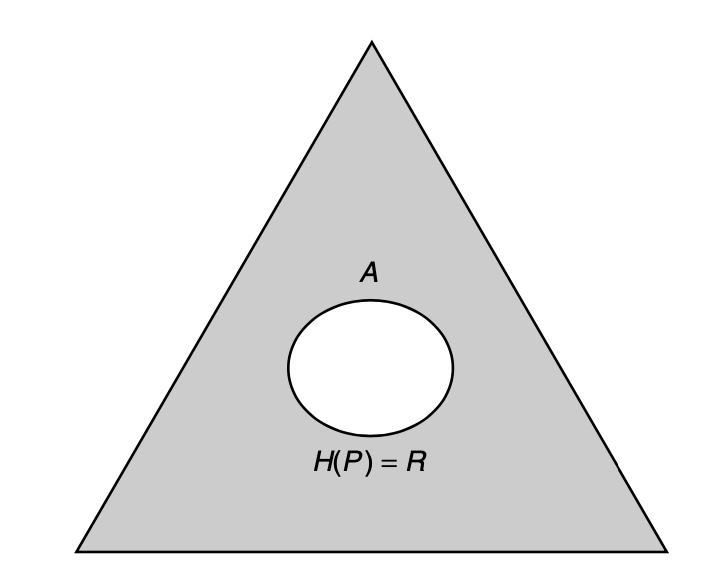
\includegraphics[width=0.5\linewidth]{Figs/fig1.png}
\centering
\caption{Universal code and the probability simplex. Each sequence with type that lies outside the circle is encoded by its index. There are fewer than $2^{nR}$ such sequences. Sequences with types \emph{within} the circle are encoded by $0$.}
		\label{un:fig1}
\end{figure}

\begin{rema}{\bfs{error exponent}}
We can get a similar lower bound from \cref{un:eq1}: $P^e_{n}\ge  Q^{n}(T(P)) $ for $P\in \{P: H(P)>R_{n}\}$, we have $P^e_{n}\ge \max_{{P: H(P)>R_{n}}} Q^{n}(T(P))\doteq 2^{nD^*_{R,Q}}$, where
\begin{align*}
D_{R, Q}^{*}=\min _{P: H(P)>R} D(P \| Q)
\end{align*}

The exponent in the probability of error is $D_{R, Q}^{*}$, which is illustrated in \cref{un:fig2}. We have: 
  \begin{align*}
       \text{ if } R&>H(Q),  D_{R, Q}^{*}>0.\\
      \text{ if } R&<H(Q), D_{R, Q}^{*}=0.
  \end{align*}
To get the exact $D_{R, Q}^{*}$ value if $R>H(Q)$, we need to use Lagrange multipliers:$$J(P)=\sum P(x) \log \frac{P(x)}{Q(x)}+\lambda \sum P(x) \log P(x)+\nu \sum P(x),$$ and differentiate with respect to $P(x)$. See \cref{ld:ema1} for a general solution.
  
\end{rema}

\begin{figure}[ht]
 \centering
 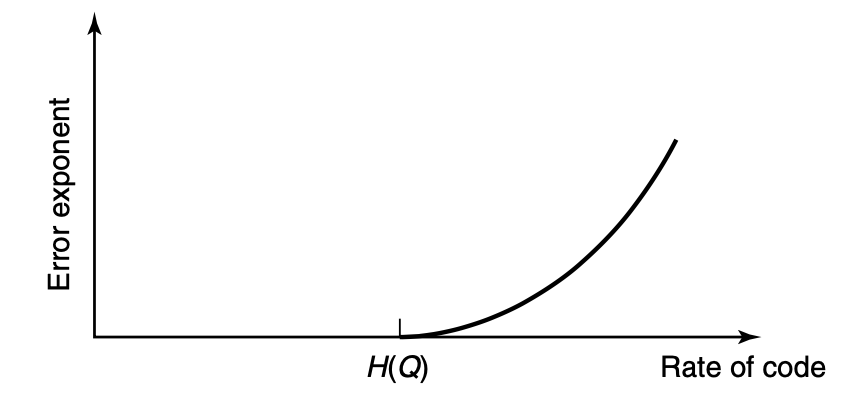
\includegraphics[width=0.5\linewidth]{Figs/fig2.png}
\centering
\caption{Error exponent for the universal code.}
		\label{un:fig2}
\end{figure}

\begin{rema}{\bfs{known distribution $Q$ or not }}
Universal codes need a longer block length to obtain the same performance as a code designed with $Q$ information. In practice if $Q$ is know, we  use Huffman codes or other code with $Q$ information
\end{rema}

\section{Large Deviation Theory}
In this section we estimate the probability of \tb{a set of nontypical types $E$}. The general idea for \tb{discrete finite} alphabet $\mathcal{X}$ is presented as Sanov's Theorem in \cref{ssect:ld_snao} which shows the sum of probability of types in $E$ is equal to the largest one to the first order in the exponent. In \cref{ssect:ld_cramer}, we present the result as Cram\'{e}r-Chernoff Theorem if $\mathcal{X}=\mathbb{R}$ (this continuous case is only considered in this section) and $E$ is specified as the empirical average deviation from the mean, i.e. $E=\{\frac{1}{n}\sum_{i=1}^n X_i>a\}$. At the first look, they have different formulation, however both of them are asymptotically tight in the exponent. In \cref{ssect:ld_equ}, we show that when $E$ is specified as the empirical average deviation from the mean, the exponent from two theorems coincide. 
\subsection{Sanov's Theorem}\label{ssect:ld_snao}

Just like what we have discussed in \cref{method:rem1} and the two important facts before \cref{sec:tv}, we will get  the sum of probability of types in $E$ is equal to the largest one to first order in the exponent, i.e. the type closest to the true distribution $Q$ in relative entropy (see \cref{method:thm4}). Note, Sanov's Theorem applies only to finite alphabets $\calX$ since the underline reason to support 
Sanov's Theorem is the two observations for \tb{discrete finite alphabets} presented before \cref{sec:tv}.

We know $\typss\subseteq \Delta_{|\calX|}$ and $\{\typss\}_{n=1}^{\infty}$ is dense, below \cref{ld:lem1} gives us how much the dense is.  
\begin{lema}{\bfs{Minimum Distance between $\calP_n$ and $P\in\Delta_{|\calX|}$}}\label{ld:lem1}
For any $P \in \Delta_{|\calX|}$,
\begin{align*}
\TV{P-\Delta_{|\calX|}} \coloneqq \inf _{Q \in\Delta_{|\calX|}} \TV{P-Q}\leq \frac{| \calX |}{2n }.
\end{align*}
\end{lema}
\begin{rema}
Sometimes we can just say $\one{P-\Delta_{|\calX|}}\leq \frac{| \calX |}{n }$
\end{rema}
\begin{proof}
 For any $P \in \Delta_{|\calX|}$, we can find a $Q \in \typss$, s.t.
\begin{align*}
|P(a)-Q(a)| \leq \frac{1}{n}, \forall a \in \calX ,
\end{align*}
because $\typss$ contains all probability vectors with component from $\left\{\frac{0}{n}, \frac{1}{n}, \ldots, \frac{n}{n}\right\}$. It follows from \cref{tv:rem2} that 
\begin{align*}
 \TV{P-Q} &=\frac{1}{2} \sum_{a \in X }|P(a)-Q(a)| \leq \frac{| \calX |}{2 n}
\end{align*}
\end{proof}


\begin{thma}{\bfs{Sanov's Theorem}}\label{ld:thm1}
Let $X_{1}, X_{2}, \ldots, X_{n}$ be \gls{iid} $\sim Q(x) .$ Let $E \subseteq \calP_n$ be a set of probability distributions. Let $E^{\circ}$ be the interior of $E$. We have
\begin{align}
-\inf _{P \in E^{\circ}} D(P \| Q) & \leq \liminf _{n \rightarrow \infty} \frac{1}{n} \log Q^n \left( E\right) \nn
& \leq \limsup _{n \rightarrow \infty} \frac{1}{n} \log Q^n\left( E\right) \nn
& \leq-\inf _{P \in E} D(P \| Q) 
\end{align}

If, in addition, the set $E$ is the closure of its interior (which implies $E$ is closed and compact, and therefore $P^{*}\in E$), then
\begin{align*}
\frac{1}{n} \log Q^{n}(E) \rightarrow-D\left(P^{*} \| Q\right)
\end{align*}
where
\begin{align}
P^{*}=\arg \min _{P \in E} D(P \| Q) \label{ld:eq1}
\end{align}
is the distribution in $E$ that is \tb{closest} to $Q$ in relative entropy (see \cref{ld:fig1}). 

\end{thma}

\begin{rema}{\bfs{upper bound of $\P(\text{set of type classes } E)$}}\label{ld:rem1}
Here we also have the upper bound
\begin{align*} 
Q^{n}(E)=Q^{n}\left(E \cap \typss\right) \leq(n+1)^{| \calX |} 2^{-n \inf _{P \in E} D(P \| Q)},
\end{align*}
Note we does not have a lower bound using $P^{*}$, for a possible lower bound we need \blue{update}. %$\arg \min _{P \in E^{\circ}} D(P \| Q)$.
\end{rema}

\begin{rema}{\bfs{achievability: $P^{*}$ in $E$ or not}}
When we say $\arg \min _{P \in E} D(P \| Q)$ instead of $\inf _{P \in E} D(P \| Q) $, it implies the achievability of the infimum in set $E$, i.e. $P^{*}\in E$.
\end{rema}

\begin{proof}
 We first prove the upper bound:
\begin{align*}
Q^{n}(E) &=\sum_{P \in E \cap \typss} Q^{n}(T(P)) \\
& \leq \sum_{P \in E \cap \typss} 2^{-n D(P \| Q)}\\
&\leq \sum_{P \in E \cap \typss} \max _{P \in E \cap \typss} 2^{-n D(P \| Q)} \\
&=\sum_{P \in E \cap \typss} 2^{-n \min _{P \in E \cap \typss} D(P \| Q)} \\
&\leq(n+1)^{| \calX |} 2^{-n \inf _{P \in E} D(P \| Q)} 
\end{align*}
We therefore get $\limsup _{n \rightarrow \infty} \frac{1}{n} \log Q^n\left( E\right) \leq-\inf _{P \in E} D(P \| Q)$.

We now come to the lower bound.
\begin{align*}
\begin{aligned}
Q^{n}(E) &=\sum_{P \in E \cap \typss} Q^{n}(T(P)) \\
& \geq \frac{1}{(n+1)^{| \calX |}} 2^{-n \min_{P\in E\cap \typss}D\left(P\| Q\right)}
\end{aligned}
\end{align*}
Consequently,
\begin{align*}
\liminf _{n \rightarrow \infty} \frac{1}{n} \log Q^n\left(E\right) \geq-\limsup _{n \rightarrow \infty} \min_{P\in E\cap \typss} D(P \| Q)
\end{align*}
For any $P\in E^{\circ}, \exists \delta>0$ s.t. $\left\{P': \TV{P'-P}<\delta\right\} \subset E$. 
From \cref{ld:lem1}, $\exists$ sequences $P_{n} \in E\cap \typss$ s.t. $P_{n} \rightarrow P$ as $n \rightarrow \infty$, we have
\begin{align*} 
-\limsup _{n \rightarrow \infty} \min_{P\in E\cap \typss} D(P \| Q)\geq-\limsup _{n \rightarrow \infty} D\left(P_{n} \| Q\right)=-D(P \| Q)
\end{align*}
Note here is $D(\cdot \| Q)$ is continuous is used. 

Since $P \in E^{\circ}$ is arbitrary, we get
\begin{align*}
\liminf _{n \rightarrow \infty} \frac{1}{n} \log Q^n\left(E\right)  \geq-\inf _{\nu \in \Gamma^{\circ}} D(\nu \| \mu)
\end{align*}
\end{proof}


\begin{figure}[ht]
 \centering
 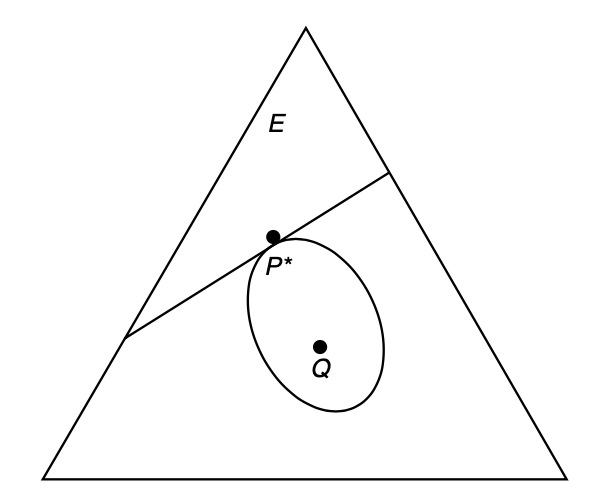
\includegraphics[width=0.5\linewidth]{Figs/fig3.png}
\centering
\caption{Error exponent for the universal code.}
		\label{ld:fig1}
\end{figure}

\begin{exma}\label{ld:ema1}
Suppose that we wish to find $Q^n\left(\left\{\frac{1}{n} \sum_{i=1}^{n} g_{j}\left(X_{i}\right) \geq \alpha_{j}, j=1,2, \ldots, k\right\}\right)$
Then the set $E$ is defined as
\begin{align*}
E=\left\{P: \sum_{a} P(a) g_{j}(a) \geq \alpha_{j}, j=1,2, \ldots, k\right\} .
\end{align*}
Using Lagrange multipliers, we construct the functional
\begin{align*}
J(P)=\sum_{x} P(x) \log \frac{P(x)}{Q(x)}+\sum_{i} \lambda_{i} \sum_{x} P(x) g_{i}(x)+v \sum_{x} P(x)
\end{align*}
We then differentiate and calculate the closest distribution to $Q$ to be of the form
\begin{align*}
P^{*}(x)=\frac{Q(x) e^{\sum_{i} \lambda_{i} g_{i}(x)}}{\sum_{a \in \calX } Q(a) e^{\sum_{i} \lambda_{i} g_{i}(a)}}
\end{align*}
where the constants $\lambda_{i}$ are chosen to satisfy the constraints. Note that if $Q$ is uniform, $P^{*}$ is the maximum entropy distribution (see tay's notes Chapter 8 Theorem 2).
\end{exma}


\begin{exma}{\bfs{joint typical set (application of \cref{ld:ema1})}}
Recall a jointly typical set is:
\begin{align*}
\begin{aligned}
A_{\epsilon}^{(n)}=\left\{\left(x^{n}, y^{n}\right) \in \calX ^{n} \times \calY ^{n}:\right.&\left|-\frac{1}{n} \log p\left(x^{n}\right)-H(X)\right|<\epsilon \\
&\left|-\frac{1}{n} \log p\left(y^{n}\right)-H(Y)\right|<\epsilon \\
&\left.\left|-\frac{1}{n} \log p\left(x^{n}, y^{n}\right)-H(X, Y)\right|<\epsilon\right\}
\end{aligned}
\end{align*}
We therefore have a $E$ as in \cref{ld:ema1}:
\begin{align*}
\begin{aligned}
E=\{P(x, y):&\left|-\sum_{x, y} P(x, y) \log Q(x)-H(X)\right| \leq \epsilon \\
&\left|-\sum_{x, y} P(x, y) \log Q(y)-H(Y)\right| \leq \epsilon \\
&\left.\left|-\sum_{x, y} P(x, y) \log Q(x, y)-H(X, Y)\right| \leq \epsilon\right\}
\end{aligned}
\end{align*}
Using Sanov's Theorem, the probability is
\begin{align*}
Q_{0}^{n}(E) \doteq 2^{-n D\left(P^{*} \| Q_{0}\right)}
\end{align*}
where $P^{*}$ is the distribution satisfying the constraints that is closest to the true distribution $Q_{0}$ in relative entropy. If we have $Q_{0}$ is the product distribution and $\epsilon \rightarrow 0$, we then have $P^{*}$ is the joint distribution $Q$ using Lagrange multipliers (set $\epsilon =0$),  so that the probability is $2^{-n D(Q(x, y) \| Q(x) Q(y))}=2^{-n I(X ; Y)}$ which is the same as the result derived for the joint AEP.
\end{exma}

\begin{exma}{\bfs{strategy to win}}
Assume there are only $n$ plays left and we must get $ n \alpha$ wins to get the final win, where $\alpha$ is much larger than the expected gain under each play. The probability that the team succeeds in achieving $ n \alpha$  points is exponentially small; hence, we can use the large deviation results and Sanov's Theorem to calculate the probability of this event. The situation is illustrated in \cref{ht:fig2}. Let $E$ be the set of types corresponding to win:
$$
E=\left\{P: \sum_{a \in \mathcal{X}} P(a) a \geq \alpha\right\}
$$
\begin{figure}[ht]
 \centering
 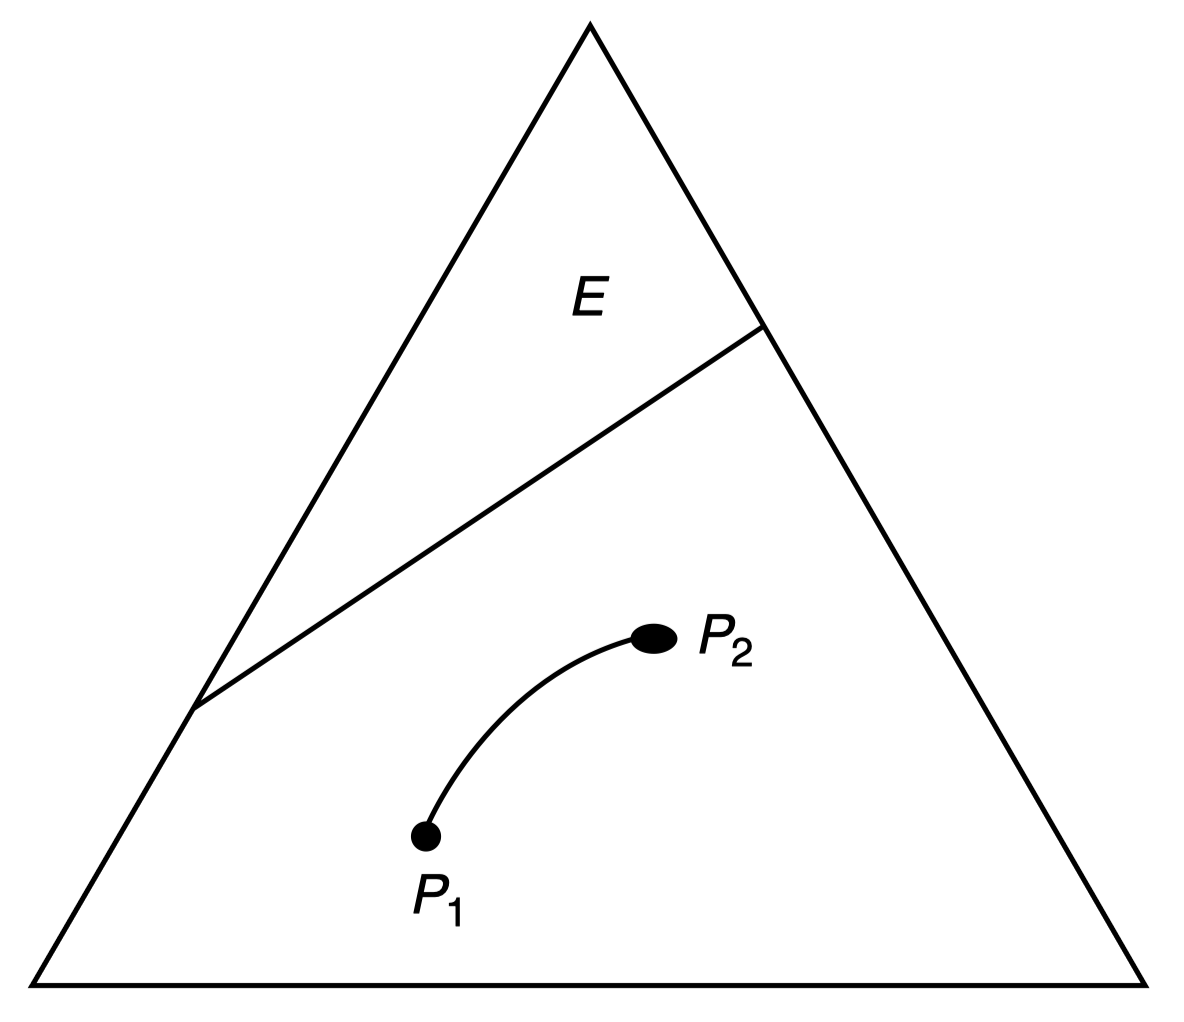
\includegraphics[width=0.5\linewidth]{Figs/fig7.png}
\centering
\caption{Strategy to win}
		\label{ht:fig2}
\end{figure}

If $P_{1}$ is gain distribution for one strategy, for types that are in $E$, we have that the final winning probability has order $2^{-n D\left(P_{1}^{*}|| P_{1}\right)}$, where $P_{1}^{*}$ is the distribution in $E$ that is closest to $P_{1}$.
If $P_{2}$ is another point distribution for another strategy, for  types that are in $E$, we have the final winning probability is that $2^{-n D\left(P_{2}^{*}|| P_{2}\right)}$. Given $P_{1}$ and $P_{2}$, we can construct a new hybrid randomized strategy $P_\lambda$: 
 $$P_\lambda = \lambda P_1 + (1-\lambda) P_2,$$
 which may have a better $2^{-n D\left(P_{\lambda}^{*}|| P_{\lambda}\right)}$.
\end{exma}

\subsection{Cram\'{e}r-Chernoff Theorem}\label{ssect:ld_cramer}
In this section we consider the case $\mathcal{X}=\mathbb{R}$.
We first give the definition of the moment generating function with some properties. We then show the definition of Fenchel-Legendre transform, and why it is useful for us. Some properties of it are then presented. In what follows, we may just write $X_1$ a $X$ if it is clear from the context.

\begin{defa}{\bfs{Moment Generating Function (MGF)}} For random variable $X$ with distributing $\mu$, the moment generating function is defined as:
$$M(\lambda)=\E{\mu}[\exp(\lambda X)]$$
\end{defa}
\blue{[a reminder to compare MGF to characteristic function or fourier transform in some notes in the future, note $\calD$ is different]}

\begin{rema}{\bfs{domain and logarithmic moment generating function}} \quad

The domain $\calD(M)$ is $\{\lambda\in \Real \mid M(\lambda) <\infty\}$.

The \tb{logarithmic moment generating function} of $X$ results from MGF by taking the $\log$:
$$\Lambda(\lambda)=\log \E{\mu}[\exp(\lambda X)]$$
\end{rema}

\begin{lema}{\bfs{Properties of MGF}}\label{ld:mgf}
The moment generating function $M(\lambda)$ of a random variable $X$ satisfies the following properties:
\begin{enumerate}[(a)]
    \item $M(0)=1$. If $M(\lambda)<\infty$ for some $\lambda>0$ then $M\left(\bar{\lambda}\right)<\infty$ for all $\bar{\lambda} \in[0, \lambda] .$ Similarly, if $M(\lambda)<\infty$ for some $\lambda<0$ then $M\left(\bar{\lambda}\right)<\infty$ for all $\bar{\lambda} \in[\lambda, 0] .$ In particular, the domain $\mathcal{D}(M)$ is an interval containing zero.
    \item Suppose $\left(\lambda_{1}, \lambda_{2}\right) \subset \mathcal{D}(M)$. Then $M(\lambda)$ as a function of $\lambda$ is differentiable in $\lambda$ for every $\lambda_{0} \in\left(\lambda_{1}, \lambda_{2}\right)$, and furthermore,
$$
\left.\frac{d}{d \lambda} M(\lambda)\right|_{\lambda=\lambda_{0}}=\mathbb{E}\left[X e^{\lambda_{0} X}\right]<\infty
$$
Namely, the order of differentiation and expectation operators can be changed.
\item More generally, we have for every $\lambda_{0} \in\left(\lambda_{1}, \lambda_{2}\right)$, and furthermore,
$$
\left.\frac{d^n}{d \lambda^n} M(\lambda)\right|_{\lambda=\lambda_{0}}=\mathbb{E}\left[X^n e^{\lambda_{0} X}\right]<\infty
$$
\end{enumerate}
\end{lema}
\begin{proof}
Part (a) is easy. We only prove part (b). Fix any $\lambda_{0} \in$ $\left(\lambda_{1}, \lambda_{2}\right)$ and consider a $\lambda$ -indexed sequence of random variables
$$
Y_{\lambda} \coloneqq \frac{\exp (\lambda X)-\exp \left(\lambda_{0} X\right)}{\lambda-\lambda_{0}}
$$
We will use the Dominated Convergence Theorem. We first identify a random variable $Z$ (better to say $Z_{\lambda_0}$) such that $\left|Y_{\lambda}\right| \leq Z$ almost surely for every $\lambda$ in some interval $\left(\lambda_{0}-\epsilon, \lambda_{0}+\epsilon\right)$, and $\mathbb{E}[Z]<\infty$. Fix $\epsilon>0$ small enough so that $\left(\lambda_{0}-\epsilon, \lambda_{0}+\epsilon\right) \subset\left(\lambda_{1}, \lambda_{2}\right) .$ We construct  
$$Z=\epsilon^{-1} \exp \left(\lambda_{0} X+\epsilon|X|\right).$$ Using the Taylor expansion of $\exp (\cdot)$ function, for every $\lambda \in\left(\lambda_{0}-\epsilon, \lambda_{0}+\epsilon\right)$, we have
$$Y_{\lambda}=\exp \left(\lambda_{0} X\right)\left(X+\frac{1}{2 !}\left(\lambda-\lambda_{0}\right) X^{2}+\frac{1}{3 !}\left(\lambda-\lambda_{0}\right)^{2} X^{3}+\cdots+\frac{1}{n !}\left(\lambda-\lambda_{0}\right)^{n-1} X^{n}+\cdots\right)$$
which gives
\begin{align*}
    \left|Y_{\lambda}\right| &\leq \exp \left(\lambda_{0} X\right)\left(|X|+\frac{1}{2!}\left(\lambda-\lambda_{0}\right)|X|^{2}+\cdots+\frac{1}{n !}\left(\lambda-\lambda_{0}\right)^{n-1}|X|^{n}+\cdots\right)\nn
&\leq \exp \left(\lambda_{0} X\right)\left(|X|+\frac{1}{2 !} \epsilon|X|^{2}+\cdots+\frac{1}{n !} \epsilon^{n-1}|X|^{n}+\cdots\right)\nn
&=\exp \left(\lambda_{0} X\right) \epsilon^{-1}(\exp (\epsilon|X|)-1)\nn
&\leq \exp \left(\lambda_{0} X\right) \epsilon^{-1} \exp (\epsilon|X|)\nn
&=Z
\end{align*}
It remains to show that $\mathbb{E}[Z]<\infty$. We have
\begin{align*}
\mathbb{E}[Z]&=\epsilon^{-1} \mathbb{E}\left[\exp \left(\lambda_{0} X+\epsilon X\right) \mathbf{1}\{X \geq 0\}\right]+\epsilon^{-1} \mathbb{E}\left[\exp \left(\lambda_{0} X-\epsilon X\right) \mathbf{1}\{X<0\}\right]\nn
&\leq \epsilon^{-1} \mathbb{E}\left[\exp \left(\lambda_{0} X+\epsilon X\right)\right]+\epsilon^{-1} \mathbb{E}\left[\exp \left(\lambda_{0} X-\epsilon X\right)\right]\nn
&=\epsilon^{-1} M\left(\lambda_{0}+\epsilon\right)+\epsilon^{-1} M\left(\lambda_{0}-\epsilon\right)\nn
&<\infty
\end{align*}
The proof is done if we note that $Y_{\lambda}\to X\exp(\lambda_0 X)$ a.s. as $\lambda \to \lambda_0$ and apply DCT.

Part (c): 
Induction is used. Fix any $\lambda_{0} \in$ $\left(\lambda_{1}, \lambda_{2}\right)$ and consider a $\lambda$ -indexed sequence of random variables
$$ 
Y_{\lambda} \coloneqq X\frac{\exp (\lambda X)-\exp \left(\lambda_{0} X\right)}{\lambda-\lambda_{0}}.
$$
From mean value theorem (in (b), we can also instead use this), we have 
$$\frac{e^{\lambda x}-e^{\lambda_{0} x}}{\lambda- \lambda_0}=x e^{(\lambda_0+h) x},$$
for a $h<\epsilon$. We therefore get that, for a small enough $\delta>0$, 
\begin{align*}
\left|x^{n+1} e^{(\lambda_0+h) x}\right| \leq\left|x^{n+1}\right| e^{(\lambda_0+\epsilon-\delta)|x|} \leq C e^{(\lambda_0+\epsilon)|x|}
\end{align*}
where $C=\max _{x} f(x)=\max _{x}\left\{|x|^{n} e^{-\delta|x|}\right\} \leq(n / \delta)^{n} e^{-n}$, which is integrable as $M(\lambda)$ is defined well at $\lambda+\epsilon$. 


\end{proof} 
\begin{lema}{\bfs{Chernoff Bound Inequality}}\label{ld:chernoffb} As an application of MGF, for any $\lambda>0$, we have
$$\P{\mu}(X>a) = \P{\mu}(\exp(\lambda X)>e^{\lambda a}) \le e^{-\lambda a}\E[\exp(\lambda X)]$$
\end{lema}
\begin{rema}
Recall that moment generate function contains the moment information of all order, we expect Chernoff Bound Inequality will get a better bound than Markov inequality (first order moment), Chebyshev inequality (second order moment) and roughly any inequality with higher order moment.

\end{rema}
\tb{introduce Fenchel-Legendre transform:}\\
We then show where Fenchel-Legendre transform comes from, its definition and why it is important.

Let $X_{1}, X_{2}, X_{3}, \ldots, X_{n}$ i.i.d. $\sim \mu$. %\in M_{1}(\mathbb{R})$
Let $\bar{S}_{n}=\frac{1}{n} \sum_{i=1}^{n} X_{i}$
From WLLN, we know $\mathbb{E}\left|X_{1}\right|<\infty$, then $\bar{S}_{n} \stackrel{p}{\rightarrow} \mathbb{E} X_{1}$ as $n \rightarrow \infty$
$\Rightarrow \mathbb{P}\left(\bar{S}_{n} \in F\right) \rightarrow 0$ as $n \rightarrow \infty$ for any closed set $F$ such that $\mathbb{E} X_{1} \notin F$. But how fast? To answer this question, we use Chernoff bound \cref{ld:chernoffb} as below:

For any $a \geq \mathbb{E} X_{1}, \lambda \geq 0$,
\begin{align}
\mathbb{P}\left(\bar{S}_{n} \geq a\right) &=\mathbb{P}\left(\exp \left(\lambda \sum X_{i}\right) \geq \exp (\lambda n a)\right) \nn
& \leq \exp (-\lambda n a) \mathbb{E}\left[\exp \left(\lambda \sum X_{i}\right)\right] \text { (Markov inequality)} \nn
&=\exp \left(-\lambda n a+\log \prod_{i} \mathbb{E}\left[\exp \left(\lambda X_{i}\right)\right]\right) \nn
&=\exp \left(-\lambda n a+\sum_{i} \log \mathbb{E}\left[\exp \left(\lambda X_{1}\right)\right]\right) \nn
&=\exp \Big(-n\{\lambda a-\Lambda(\lambda)\}\Big)\\
\end{align}
To get the best bound, we take sup over $\lambda$ :
\begin{align}
\mathbb{P}\left(\bar{S}_{n} \geq a\right) \leq \exp \left(-n \sup _{\lambda \geq 0}\{\lambda a-\Lambda(\lambda)\}\right) \label{ld:ca:1}
\end{align}
\begin{defa}{\bfs{Fenchel-Legendre Transform}}
The Fenchel-Legendre transform of $\Lambda(\lambda)$ is defined as
\begin{align}
I(x)=\sup _{\lambda \in \mathbb{R}}\{\lambda x-\Lambda(\lambda)\} \label{ld:ca:2}
\end{align}
\end{defa}
\begin{rema}{\bfs{a summary of concepts}}
\begin{enumerate}
    \item MGF: $M(\lambda)=\E{\mu}[\exp(\lambda X)]$
    \item logarithmic moment generating function: $\Lambda(\lambda)=\log M(\lambda)$
    \item Fenchel-Legendre transform: $I(x)=\sup _{\lambda \in \mathbb{R}}\{\lambda x-\Lambda(\lambda)\}$
    
    Note here Fenchel-Legendre transform is a supremum over a set of linear function so it is convex, this property is prove rigorously in \cref{ld:lemfen}.
    
    Note in the definition of Fenchel-Legendre transform the \tb{supremum is taken over $\Real$ not just non-negative real value.} However, we will show in  \cref{ld:thm_cramer} that $\sup _{\lambda \geq 0}\{\lambda a-\Lambda(\lambda)\}$ can be safetly replaced by $I(x)$ when  $a \geq \mathbb{E} X_{1}$.
\end{enumerate}
\end{rema}


\begin{lema}{\bfs{Properties of Fenchel-Legendre Transform}}\label{ld:lemfen}Assume $\Lambda(\lambda) < \infty$ for all $\lambda \in \mathbb{R}$ (i.e. $\calD =\Real$), we next present several properties of $I(x)$:
\begin{enumerate}[(a)]
    \item $\Lambda$ and $I$ are convex.
    \item $I(\cdot)$ is lower semi-continuous with
        \begin{itemize}
            \item $I(\E[X_1])=0$ and $I(x) \geq 0 \quad \forall x$
            \item $I(x)=\sup\limits_{\lambda\geq0}\{\lambda x-\Lambda(\lambda)\}$ for $x \geq \E[X_1]$
			\item $I(x)=\sup\limits_{\lambda\leq0}\{\lambda x-\Lambda(\lambda)\}$ for $x < \E[X_1]$
        \end{itemize}
    \item $I$ is a decreasing function on $(-\infty, \E[X_1]]$, and an increasing function on  $[\E[X_1], +\infty)$
    
        	\item  $\Lambda$ is differentiable with
	\begin{align*}
		\Lambda'(\lambda)=\frac{1}{\E[\exp(\lambda X_1)]}\E[X_1 \exp(\lambda X_1)]
	\end{align*}
	If we have 	$\Lambda'(\lambda_0)=x_0 $ for one pair $(\lambda_0,x_0)$, this $\lambda_0$ is the one achieve the supremum in $I(x_0)$, i.e.
	\begin{align*}	
		 I(x_0)= \lambda_0 x -\Lambda(\lambda_0)
	\end{align*}
	Furthermore for any $x_0$ we can find one $\lambda_0$ such that $\Lambda'(\lambda_0)=x_0 $, i.e. the supremum is a achievable maximum with one $\lambda_0$.
	\item We have the conclusion for the second order derivative:
	\begin{align*}
		\Lambda''(\lambda)=\E_{\lambda}[X^2] - (\E_{\lambda}[X])^2, \text{ where we define } \E_{\lambda}[f(X)]\coloneqq \frac{\E[f(X)e^{\lambda X}]}{\E[e^\lambda X]}
	\end{align*}
\end{enumerate}
\begin{rema}\bfs{exponential family}
	In sum, we can define a probability measure $\nu_{\lambda_0}$ on $\mathbb{R}$ by
			\begin{align*}
			\nu_{\lambda_0}(A)=\frac{1}{\E[\exp(\lambda_0 X_1)]}\int_{A}\exp(\lambda x)\ud \mu\ \ \forall A \in\mathbb{B}(\mathbb{R})
			\end{align*}
		and a random variable $Y\sim \nu_{\lambda_0}$, so that we get
		$$	\Lambda'(\lambda) =\E [Y] \text{ and } \Lambda''(\lambda)=\mathrm{var}[Y].$$
	The more general theorem is presented in \cite[Theorem 1.6.2.]{Statistics}.
\end{rema}
\end{lema} 
	\begin{proof}$\ $\\
	\begin{enumerate}[label=(\alph*)]
	\item
		\begin{align*}
		   \Lambda(\theta\lambda_1+(1-\theta)\lambda_2)& =\log\E[(\exp(\lambda_1 X_1))^\theta (\exp(\lambda_2X_1))^{1-\theta}] \\
		   & \leq\log\E\left([\exp(\lambda_1 X_1)]\right)^\theta\left(\E[\exp(\lambda_2 X_2)]\right)^{1-\theta} \\
		   & =\theta\Lambda(\lambda_1)+(1-\theta)\Lambda(\lambda_2)
		\end{align*}
		Hint: H{\"o}lder's inequality: $\E|XY|\leq(\E|X|^p)^{\frac{1}{p}} (\E|Y|^q)^{\frac{1}{q}}$ when $\frac{1}{p}+\frac{1}{q}=1$
		\begin{align*}
		   I(\theta x_1+(1-\theta)x_2)
		   &=\sup\limits_{\lambda\in\mathbb{R}}\{\lambda(\theta x_1+(1-\theta)x_2)-\Lambda(\lambda)\}\\
		   &\leq \sup\limits_{\lambda\in\mathbb{R}}\{\lambda\theta x_1-\theta\Lambda(\lambda)\}+\sup\limits_{\lambda\in\mathbb{R}}\{\lambda(1-\theta)x_2-(1-\theta)\Lambda(\lambda)\}\\ &=\theta I(x_1)+(1-\theta)I(x_2)
		\end{align*}
	\item
		Let $x_n\rightarrow x$ as $n\rightarrow\infty $. For any $\lambda\in\mathbb{R}$
		\begin{align*}
		  \liminf\limits_{x_n\rightarrow x} I (x_n)& \geq\liminf\limits_{x_n\rightarrow x}(\lambda x_n-\Lambda(\lambda))\\
		  &=\lambda x-\Lambda(\lambda).
		\end{align*}
	We therefore have 
		\begin{align*}
		  \liminf\limits_{x_n\rightarrow x} I (x_n)& \geq\sup\limits_{\lambda\in\mathbb{R}}(\lambda x-\Lambda(\lambda))\\
		  &=I(x)
		\end{align*}
		Thus, $I$ is lower semi-continuous. From the definition of $I(x)$ by taking a $\lambda =0$, we have
		\begin{align*}
		I(x)\geq  -\Lambda(0)=0\ \ \forall x
		\end{align*}
		For any $\lambda \in \mathbb{R}$,
		\begin{align*}
		\Lambda(\lambda)&=\log\E[\exp(\lambda X_1)]\\
		&\geq\E[\log(\exp(\lambda X_1))]\\
		&=\lambda \E[X_1]
		\end{align*}
	We therefore have $I(\E[X_1])\leq 0$. Together with $	I(x)\geq  -\Lambda(0)=0\ \ \forall x$, we have $I(\E[X_1])=0$.
	
	We next prove the other two conlusion:
	
	If $x\geq\E[X_1]$ , for $\lambda<0$,\\
		\begin{align*}
		\lambda &x-\Lambda(\lambda)\leq\lambda\E[X_1]-\Lambda(\lambda)\leq I(\E[X_1])=0\\
		&\Rightarrow I(x)=\sup\limits_{\lambda\geq0}[\lambda x-\Lambda(\lambda)]
		\end{align*}
		The proof is similar for $x<\E[X_1]$.
	\item  The monotonicity follows from convexity of $\Lambda$ and  $I(x)\ge I (\E[X_1])$.
	\item
		From \cref{ld:mgf} (b), we have $\Lambda'(\lambda) = (\log M(\lambda))'= \frac{M'(\lambda)}{M(\lambda)]} = \frac{1}{M(\lambda)}\E[X\exp(\lambda X)]$.
		
		Since $\Lambda(\lambda)$ is convex, we have $\lambda x - \Lambda(\lambda)$  is concave, we therefore only need to prove 
		$$
\lim _{|\lambda| \rightarrow \infty} \theta x-\log M(\lambda)=-\infty.
$$
		For any $K>0$ we have
$$
\begin{aligned}
\liminf _{\lambda \rightarrow \infty} \frac{\log M(\lambda)}{\lambda} &=\liminf _{\lambda \rightarrow \infty} \frac{\log \left(\int \exp (\lambda x) \mathrm{d} P(x)\right)}{\lambda} \\
& \geq \liminf _{\lambda \rightarrow \infty} \frac{1}{\lambda} \log \left(\int_{K}^{\infty} \exp (\lambda x) \mathrm{d} P(x)\right) \\
& \geq \liminf _{\lambda \rightarrow \infty} \frac{1}{\lambda} \log (\exp (K \lambda) \mathbb{P}([K, \infty])) \\
&=K+\liminf _{\lambda \rightarrow \infty} \frac{1}{\lambda} \log \mathbb{P}([K, \infty]) \\
&=K\left(\text { since } \operatorname{supp}\left(X_{1}\right)=\mathbb{R}, \text { we have } \mathbb{P}([K, \infty))>0 .\right)
\end{aligned}
$$
Since $K$ is arbitrary,
$$
\liminf _{\lambda \rightarrow \infty} \frac{1}{\lambda} \log M(\lambda)=\infty
$$
Similarly,
$$
\liminf _{\lambda \rightarrow-\infty}-\frac{1}{\lambda} \log M(\lambda)=\infty
$$
Therefore,
$$
\lim _{\lambda \rightarrow \infty} \lambda x-\log M(\lambda)=\lim _{\lambda \rightarrow \infty} \lambda\left(x-\frac{1}{\lambda} \log M(\lambda)\right) \rightarrow-\infty
$$
Therefore, for each $x$ as $|\lambda| \rightarrow \infty$, we have that
$$
\lim _{|\lambda| \rightarrow \infty} \lambda x-\log M(\lambda)=-\infty
$$

		
\item Please 	see the proof for (ii) in \cref{ld:thm_cramer}, where the new random variable $Y$ is defined as the key. 	
		
		
		
	\end{enumerate}
	\end{proof}

Let
		\begin{align*}
		\alpha=\inf\{x\in\mathbb{R}:\mu((-\infty,x])>0\}\\
		\beta=\sup\{x\in\mathbb{R}:\mu([x,\infty))>0\}
		\end{align*}

\begin{thma}{\bfs{Cramer's Theorem }}\label{ld:thm_cramer}
 Suppose $X_1,X_2,...,X_n\overset{i.i.d.}{\thicksim}\mu$, and let $\bar{S}_n=\frac{1}{n}\sum_{i=1}^{n}X_i$.
	\begin{enumerate}[label=(\roman*)]
	\item
	\begin{align*}
	\P(\bar{S}_n\geq a)\leq \exp(-nI(a))\ for\ all\ a\geq\E[X_1]\\
	\P(\bar{S}_n\leq a)\leq \exp(-nI(a))\ for\ all\ a\leq\E[X_1]
	\end{align*}
	\item
	 For $a\in(\alpha,\beta),\epsilon>0,$
	\begin{align*}
	\P(|\bar{S}_n- a|<\varepsilon)\geq \left(1-\frac{\Lambda^{''}(\lambda_0)}{n\epsilon^{2}}\right)\exp(-n(I(a)+\epsilon|\lambda_0|))
	\end{align*}
	where $\lambda_0$ is s.t. $\Lambda'(\lambda_0)=a$ (i.e. $I(a)=\lambda_0 a-\Lambda(\lambda_0)$).
	\end{enumerate}
\end{thma}

\begin{proof}$\ $
	\begin{enumerate}[label=(\roman*)]
		\item The first inequality comes directly from applying \cref{ld:lemfen}. To get the second inequality, we have
		\begin{align*}
		    \P(\bar{S}_n\leq a)&= \P(-\bar{S}_n\geq -a)\\
		    &\le \exp\bigg(-n\sup_{\lambda\ge 0 } \{-\lambda a- \Lambda(-\lambda)\}\bigg)\\
		    &= \exp\bigg(-n\sup_{\bar{\lambda}\le 0 } \{\bar{\lambda} a- \Lambda(\bar{\lambda})\}\bigg)\\
		    &= \exp\bigg(-nI(a)\bigg)
		\end{align*}
		
		\item Suppose $a\geq\E[X_1]$, then from \cref{ld:lemfen}, $\lambda_0\geq0$,
			Define a probability measure $\nu_{\lambda_0}$ on $\mathbb{R}$ by
			\begin{align*}
			\nu_{\lambda_0}(A)=\frac{1}{\E[\exp(\lambda_0 X_1)]}\int_{A}\exp(\lambda x)\ud \mu\ \ \forall A \in\mathbb{B}(\mathbb{R})\\
			\Rightarrow \frac{\ud\nu_{\lambda_0}}{\ud\mu}=\exp\bigg((\lambda_0 x)-\Lambda(\lambda_0)\bigg)\ \ \mbox{(exponential tilting)}
			\end{align*}
			Let $Y_1,Y_2,Y_3,...,Y_n\overset{i.i.d.}{\thicksim}\nu_{\lambda_0},\ \bar{T}_n=\frac{1}{n}\sum_{i=1}^{n}Y_i$,
			\begin{align*}
			\P(|\bar{S}_n-a|<\varepsilon)
			&=\int_{A}\mu(d x_1)...\mu(d x_n)\ \mbox{where}\ A=\left\{x^n:|\sum_{i=1}^{n}x_i-na|<n\varepsilon\right\}\\
			&=\int_{A}\exp\bigg(-(\lambda_0\sum x_i-n\Lambda(\lambda_0))\bigg)\nu_{\lambda_0}(d x_1)...\nu_{\lambda_0}(d x_n)\\
			&\geq\exp\bigg(-(\lambda_0 n(a+\varepsilon)-n\Lambda(\lambda_0)\bigg))\P{\nu_{\lambda_0}}(|\bar{T}_n-a|<\varepsilon)\\
			&=\exp(-n(I(a)+\varepsilon\lambda_0))\P{\nu_{\lambda_0}}(|\bar{T}_n-a|<\varepsilon) 
			\end{align*}
			Since
			\begin{align*}
			\E{\nu_{\lambda_0}}[\bar{T}_n] &= \ \E{\nu_{\lambda_0}}[Y_1]\\
			&=\int_{\mathbb{R}}x\exp\bigg(\lambda_0 x-\Lambda(\lambda_0)\bigg)\ud\mu\\
			&=\frac{1}{\E_\mu[\exp(\lambda_0 X)]}\E_\mu[X_1\exp(\lambda_0 X_1)]\\
			&=\Lambda'(\lambda_0) \ \mbox{from Lemma \cref{ld:lemfen}}\\
			&=a
			\end{align*}
			We obtain from Chebyshev's inequality that 
			\begin{align*}
			\P(|\bar{S}_n-a|<\varepsilon)
			&\geq\exp\bigg(-n(I(a)+\varepsilon\lambda_0)\bigg)\bigg(1-\frac{\var_{\nu_{\lambda_0}}(\bar{T}_n)}{\varepsilon^{2}}\bigg)\\
			&=\bigg(1-\frac{\Lambda''(\lambda_0)}{n\varepsilon^2}\bigg)\exp\bigg(-n(I(a)+\varepsilon\lambda_0)\bigg),
			\end{align*}
			where we use the fact 
			\begin{align*}
			\var_{\nu_{\lambda_0}}(\bar{T}_n)
			&=\frac{1}{n} \var_{\nu_{\lambda_0}}(Y_1)\\
			&=\frac{1}{n}\Lambda''(\lambda_0).
			\end{align*}
			The last equality follows since: We know $\mathbb{E}Y = \frac{M’}{M}=\Lambda’$.
We also easily get $\Lambda''$ $=\frac{M''M-(M’)^2}{M^2}$. As $\mathrm{Var}(Y) = \E (Y^2)- (EY)^2=\E (Y^2) - (\frac{M’}{M})^2$, we then need to prove $\E Y^2 = \frac{MM''}{M^2}=\frac{M''}{M}$, which is correct from \cref{ld:mgf} (c).

			Similar proof for $a<\E[X_1]$, and proof is completed.  
	\end{enumerate}  
\end{proof}

\begin{rema}{\bfs{change of measure method}}
The argument used in proof above is a ``change of measure'' method, which proves to be very useful in various applications.
\end{rema}
\begin{rema}{\bfs{generalized Cramer's Theorem}}
Cramer's Theorem can be generalized as follows:
\begin{enumerate}[label=(\roman*)]
\item For any closed set $F\subseteq\mathbb{R}$
	\begin{align*}
	\limsup\limits_{n\rightarrow\infty}\frac{1}{n}\log\P(\bar{S}_n\in F)\leq-\inf\limits_{x\in F}I(x).
	\end{align*}
\item For any open set $G\subseteq\mathbb{R}$
	\begin{align*}
	\liminf\limits_{n\rightarrow\infty}\frac{1}{n}\log\P(\bar{S}_n\in G)\geq-\inf\limits_{x\in G}I(x).
	\end{align*}
\end{enumerate}
An intuitive understanding is the set $F$ and $G$ can be covered by $(-\infty, z^-]$ and $[z^+, \infty) $ for some $z^-<\E[X_1]<z^+$, and $I$ is a decreasing function on $(-\infty, \E[X_1]]$, and an increasing function on  $[\E[X_1], +\infty)$. So the infinum is at $ z^- $ or $ z^+$. 
\end{rema}


\begin{cora}
For any $a\in\mathbb{R}$
\begin{align*}
\lim_{n\rightarrow\infty}\frac{1}{n}\log\P(\bar{S}_n\geq a)=-\inf\limits_{x\geq a}I(x).
\end{align*}
\end{cora}
\begin{proof}
	Suppose a$\geq \E[X_1]$. From Cramer's Theorem,
	\begin{align*}
		\limsup_{n\rightarrow\infty}\frac{1}{n}\log\P(\bar{S}_n\geq a)&\leq-I(a)\\
		\liminf_{n\rightarrow\infty}\frac{1}{n}\log\P(\bar{S}_n\geq a)
		&\geq\liminf\limits_{n\rightarrow\infty}\frac{1}{n}\log\P(\bar{S}_n\geq a+\varepsilon)\ \ \forall \varepsilon>0\\
		&\geq-I(a)-\varepsilon|\eta|	
	\end{align*}
	Take $\varepsilon\rightarrow0$, we get $\lim\limits_{n\rightarrow\infty}\frac{1}{n}\log\P(\bar{S}_n\geq a)=-I(a)$\\
	If $a<\E[X_1]$, from WLLN,$P(\bar{S}_n\geq a)\rightarrow1$ and
	\begin{align*}
		\lim\limits_{n\rightarrow\infty}\frac{1}{n}\log\P(\bar{S}_n\geq a)=0=-I(\E[X_1])=-\inf\limits_{x\geq a}I(x)
	\end{align*}

\end{proof}


\subsection{Sanov's Theorem vs. Cram\'{e}r-Chernoff Theorem}\label{ssect:ld_equ}

We know Cram\'{e}r-Chernoff Theorem can work even when $\mathcal{X}=\mathbb{R}$. We of source can still apply Cram\'{e}r-Chernoff Theorem to  discrete finite alphabet $\mathcal{X}$, which will get an exponent. In this section, we still only consider $E$ is specified as the empirical average deviation from the mean, i.e. $E=\{\frac{1}{n}\sum_{i=1}^n X_i\ge a\}$.

It turns out that the Cramér-Chernoff Theorem and Sanov's Theorem shows the same exponent over $E$. 
We need to evaluate $D\left(P \| Q\right)$ in this case, which can be done as follows:
\begin{enumerate}
    \item Introduce a Lagrange multiplier to obtain:
$$
\min _{P \in E} D\left(P \| Q\right)=\min _{\left\{P \mid \E{P}[X] \geq a\right\}} D\left(P \| Q\right)=\min _{P} \sup _{\lambda>0}\left\{D\left(P \| Q\right)-\lambda\left(\E{P}[X]-a\right)\right\}
$$
\item Use Von Neumann's minimax theorem to swap the order of the min and the sup:
$$
\min _{P} \sup _{\lambda>0}\left\{D\left(P \| Q\right)-\lambda\left(\E{P}[X]-a\right)\right\}=\sup _{\lambda>0} \inf _{P}\left\{D\left(P \| Q\right)-\lambda\left(\E{P}[X]-a\right)\right\}
$$
\item Recognize the following convex duality for Kullback-Leibler divergence:
$$
\sup _{P}\left(\E{P}[\lambda X]-D\left(P|| Q\right)\right)=\mu(\lambda)
$$
where $\mu(\lambda)=\log \E{Q}\left[e^{\lambda X}\right]$ is the cumulant generating function defined above. We get:
$$
\begin{aligned}
\sup _{\lambda>0} \inf \left\{D\left(P \| Q\right)-\lambda\left(\E{P}[X]-a\right)\right\} &=\sup _{\lambda>0}\left\{\lambda a-\sup _{P}\left(\E{P}[\lambda X]-D\left(P \| Q\right)\right)\right\} \\
&=\sup _{\lambda>0}\{\lambda a-\mu(\lambda)\}
\end{aligned}
$$
Chaining everything together we exactly recover the Cramér-Chernoff theorem, and we see that the upper bounds have exactly the same constants.
\end{enumerate}

\tb{Summary:}\\
% We summarized as 
\begin{enumerate}
    \item Sanov's Theorem only deals with \tb{discrete finite} alphabet $\mathcal{X}$.
    \item  Cram\'{e}r-Chernoff Theorem deals with discrete finite alphabet $\mathcal{X}$ and continuous $\mathcal{X}$ like  $\mathcal{X}=\Real$
    \item Both theorems can be applied to get asymptotic probability exponent, and both can be applied to get finite samples. (In \cref{ssect:ld_snao}, the Sano's Theorem only focuses on the asymptotic behavior, however we can still use the inequality shown in the proof to provide finite samples inequality.
    \item In \tb{discrete finite} alphabet case, Sanov's Theorem and  Cram\'{e}r-Chernoff Theorem have the same asymptotic exponent which is expected since the same event cannot have two different probability exponent.
\end{enumerate}

\section{Conditional Limit Theorem}\label{sec:clt}
In the last section we have shown that $Q^n(E)$ essentially determined by $D\left(P^{*}|| Q\right)$, the distance of the \tb{closest} element of $E$ to $Q$. In this section we shown that given that we are in set $E$, the type  $P_{X^n}$ is very likely to be close to $P^{*}$. The \tb{main idea} is $P^*$ is the dominant term in $E$, given $E$, $P_{X^n}$ observed is close to $P^*$. 

We first prove a ``Pythagorean'' theorem of relative entropy which is  analogous to square of the Euclidean distance. After this, we prove the Conditional limit theorem. 
\begin{figure}[ht]
 \centering
 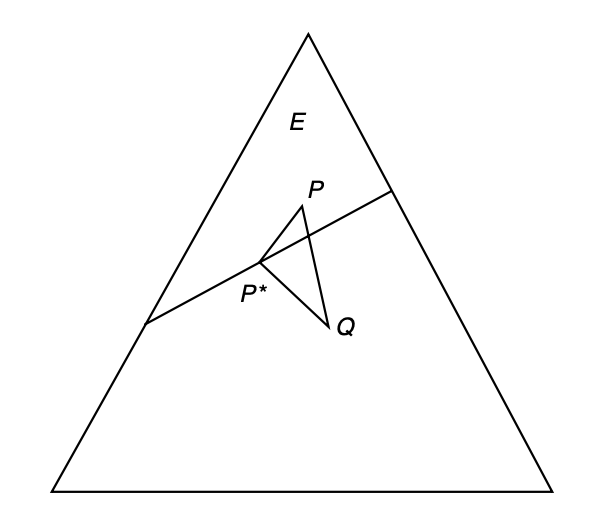
\includegraphics[width=0.5\linewidth]{Figs/fig4.png}
\centering
\caption{Pythagorean theorem for relative entropy.}
		\label{ld:fig4}
\end{figure}

\begin{thma}{\bfs{``Pythagorean'' Theorem}}\label{clt:thm1}
For a closed convex set $E \subset P$ and distribution $Q \notin$ $E$, let $P^{*} \in E$ be the distribution that achieves the minimum distance to $Q$; that is,
\begin{align*}
D\left(P^{*} \| Q\right)=\min _{P \in E} D(P \| Q)
\end{align*}
Then
\begin{align*}
D(P \| Q) \geq D\left(P \| P^{*}\right)+D\left(P^{*} \| Q\right)
\end{align*}
for all $P \in E$.
\end{thma}
\begin{rema}{\bfs{closed and convex}}\label{clt:rem2}
``Closed'' guarantees $P^* \in E$, while the convex condition is also important for  ``$P_\lambda\in E$'' in the very beginning of the  proof, i.e. it is essential for \cref{clt:thm1}.
\end{rema}
\begin{rema}{\bfs{main use of \cref{clt:thm1}}}\label{clt:rem3}
Suppose that we have a sequence $P_{n} \in E$ that yields $D\left(P_{n}|| Q\right) \rightarrow D\left(P^{*} \| Q\right)$. Then from the Pythagorean theorem, $D\left(P_{n} \| P^{*}\right) \rightarrow 0$ as well.
\end{rema}
\begin{rema}{\bfs{analogy to square of the Euclidean distance}}\label{clt:rem4}
Note that the relative entropy $D(P \| Q)$ behaves like the square of the Euclidean distance.
\end{rema}
\begin{proof}
 Consider any $P \in E$. Let
\begin{align*}
P_{\lambda}=\lambda P+(1-\lambda) P^{*}
\end{align*}
Then $P_{\lambda} \rightarrow P^{*}$ as $\lambda \rightarrow 0$. Also, since $E$ is convex, $P_{\lambda} \in E$ for $0 \leq \lambda \leq 1$. Since $D\left(P^{*}|| Q\right)$ is the minimum of $D\left(P_{\lambda} \| Q\right)$ along the path $P^{*} \rightarrow P$, the derivative of $D\left(P_{\lambda} \| Q\right)$ as a function of $\lambda$ is nonnegative at $\lambda=0$. Now
\begin{align*}
D_{\lambda}=D\left(P_{\lambda} \| Q\right)=\sum P_{\lambda}(x) \log \frac{P_{\lambda}(x)}{Q(x)}
\end{align*}
and
\begin{align*}
\frac{d D_{\lambda}}{d \lambda}=\sum\left(\left(P(x)-P^{*}(x)\right) \log \frac{P_{\lambda}(x)}{Q(x)}+\left(P(x)-P^{*}(x)\right)\right)
\end{align*}
Setting $\lambda=0$, so that $P_{\lambda}=P^{*}$ and using the fact that $\sum P(x)=\sum P^{*}(x)=1$, we have
\begin{align}
% \begin{aligned}
0 & \leq\left(\frac{d D_{\lambda}}{d \lambda}\right)_{\lambda=0} \label{clt:eq1}\\
&=\sum\left(P(x)-P^{*}(x)\right) \log \frac{P^{*}(x)}{Q(x)} \nn
&=\sum P(x) \log \frac{P^{*}(x)}{Q(x)}-\sum P^{*}(x) \log \frac{P^{*}(x)}{Q(x)} \nn
&=\sum P(x) \log \frac{P(x)}{Q(x)} \frac{P^{*}(x)}{P(x)}-\sum P^{*}(x) \log \frac{P^{*}(x)}{Q(x)} \nn
&=D(P \| Q)-D\left(P \| P^{*}\right)-D\left(P^{*} \| Q\right)
% \end{aligned}
\end{align}
which proves the theorem.
\end{proof}
\begin{rema}{\bfs{necessary and sufficient condition for minimum $x^{*}$ in convex optimization}}\label{clt:rem5}
(This remark serves as a reminder only, other readers can ignore this.) The tangent cone of convex domain $M$ at $x^{*}$ is the cone
\begin{align*}
T_{M}\left(x^{*}\right)=\left\{h \in R ^{n} \mid x^{*}+t h \in M \quad \forall \text { small enough } t>0\right\}
\end{align*}
For the  convex  function $f$ on $M$ which is differentiable at $x^{*}$ the necessary and sufficient condition for $x^{*}$ to be a minimizer of $f$ on $M$ is :
$(*)$ the derivative of $f$ taken at $x^{*}$ along every direction from $T_{M}\left(x^{*}\right)$ should be nonnegative:
\begin{align*}
h^{T} \nabla f\left(x^{*}\right) \geq 0 \quad \forall h \in T_{M}\left(x^{*}\right)
\end{align*}
% In our case, the above can be used to directly get \cref{clt:eq1}. %Note $f'$ cannot have any simple discontinuities.
\end{rema}

\tb{Outline of the proof}:
We can now begin the proof of the conditional limit theorem. We first outline the method used. Since the probability of a type under $Q$ depends exponentially on the distance of the type from $Q$, and hence types that are farther away are exponentially less likely to occur. 
We divide the set of types in $E$ into two categories as shown in \cref{clt:fig5}: 
\begin{enumerate}
    \item Types that are at about the same distance from $Q$ as $P^{*}$.
    \item Types that are at a distance $2 \delta$ farther away.
\end{enumerate}
The second set has exponentially less probability than the first, and hence the first set has a conditional probability tending to $1$ . We then use the Pythagorean theorem to establish that all the elements in the first set are close to $P^{*}$, which will establish the theorem.
\begin{figure}[ht]
 \centering
 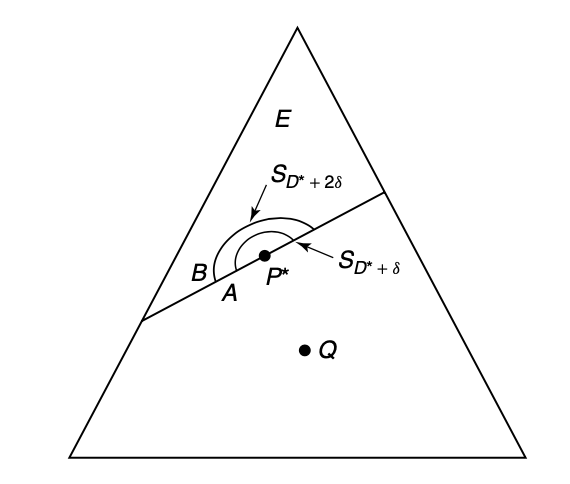
\includegraphics[width=0.5\linewidth]{Figs/fig5.png}
\centering
\caption{Conditional limit theorem.}
		\label{clt:fig5}
\end{figure}


\begin{thma}{\bfs{Conditional limit theorem}}\label{clt:thm2}
Let $E$ be a closed convex subset of $P$ and let $Q$ be a distribution not in $E .$ Let $X_{1}, X_{2}, \ldots, X_{n}$ be discrete random variables drawn i.i.d. $\sim Q .$ Let $P^{*}$ achieve $\min _{P \in E}$ $D(P \| Q) .$ Then for all $a\in calX$
\begin{align*}
Q^n\left(X_{1}=a \mid P_{X^{n}} \in E\right) \rightarrow P^{*}(a) \text{ as } n \rightarrow \infty. 
\end{align*}
In other words, the conditional distribution of $X_{1}$, given that the type of the sequence is in $E$, is close to $P^{*}$ for large $n$.
\end{thma}

\begin{rema}{\bfs{why convex and closed}}
    Convex and closed is essential for \cref{clt:thm1} as we have discussed in \cref{clt:rem2}. One additional property I need to mention is that strictly convex of $D(\cdot \| Q)$ ensures the uniqueness of $P^*$ which is also important for the correctness of  \cref{clt:thm1}.
\end{rema}

\begin{rema}{\bfs{weak convergence}}
    \cref{clt:thm1} indicates PMF converges for each $a\in \calX$. $P^{*}$ is also a discrete distribution. So we have conditional distribution of $X_{1}$ converge to $P^{*}$ in distribution (weak convergence).
\end{rema}

\begin{proof}
We define convex set $S_{t}$ as 
$S_{t}=\{P \in P : D(P \| Q) \leq t\}
$ and let 
$D^{*}=D\left(P^{*} \| Q\right)$. 
We now formally define the two sets as we have outlined in the discussion before \cref{clt:thm1}:
\begin{enumerate}
    \item $A=S_{D^{*}+2 \delta} \cap E$
    \item $ B=E-S_{D^{*}+2 \delta} \cap E$
\end{enumerate}
Thus, $A \cup B=E .$ These sets are illustrated in \cref{clt:fig5}. Then
\begin{align*}
\begin{aligned}
Q^{n}(B) &=\sum_{P \in E \cap \typss: D(P \| Q)>D^{*}+2 \delta} Q^{n}(T(P)) \\
& \leq \sum_{P \in E \cap \typss: D(P \| Q)>D^{*}+2 \delta} 2^{-n D(P \| Q)} \\
& \leq \sum_{P \in E \cap \typss: D(P|| Q)>D^{*}+2 \delta} 2^{-n\left(D^{*}+2 \delta\right)} \\
& \leq(n+1)^{| \calX |} 2^{-n\left(D^{*}+2 \delta\right)}
\end{aligned}
\end{align*}
On the other hand,
\begin{align*}
\begin{aligned}
Q^{n}(A) & \geq Q^{n}\left(S_{D^{*}+\delta} \cap E\right)  \text{ (note here is $\delta$) }\\
&=\sum_{P \in E \cap \typss: D(P \| Q) \leq D^{*}+\delta} Q^{n}(T(P)) \\
& \geq \sum_{P \in E \cap \typss: D(P \| Q) \leq D^{*}+\delta} \frac{1}{(n+1)^{| \calX |}} 2^{-n D(P \| Q)}\\
&\geq \frac{1}{(n+1)^{| \calX |}} 2^{-n\left(D^{*}+\delta\right)} \text{ for sufficiently large $n$ }
\end{aligned}
\end{align*}

since the sum is greater than one of the terms, and for sufficiently large $n$, there exists at least one type in $S_{D^{*}+\delta} \cap E \cap \typss$ (recall  $\typss$ is dense). Then, for $n$ sufficiently large,
\begin{align*}
\begin{aligned}
\operatorname{Pr}\left(P_{X^{n}} \in B \mid P_{X^{n}} \in E\right) &=\frac{Q^{n}(B \cap E)}{Q^{n}(E)} \\
& \leq \frac{Q^{n}(B)}{Q^{n}(A)} \\
& \leq \frac{(n+1)^{| \calX |} 2^{-n\left(D^{*}+2 \delta\right)}}{\frac{1}{(n+1)^{| \calX |}} 2^{-n\left(D^{*}+\delta\right)}} \\
&=(n+1)^{2| \calX |} 2^{-n \delta},
\end{aligned}
\end{align*}


which goes to 0 as $n \rightarrow \infty$. Hence the conditional probability of $B$ goes to 0 as $n \rightarrow \infty$, which implies that the conditional probability of $A$ goes to $1 .$

We now show that all the members of $A$ are close to $P^{*}$ in relative entropy. For all  $P\in A$, from \cref{clt:thm1} we have
\begin{align*}
D\left(P \| P^{*}\right)+D\left(P^{*} \| Q\right) \leq D(P \| Q) \leq D^{*}+2 \delta
\end{align*}
which implies that
\begin{align*}
D\left(P \| P^{*}\right) \leq 2 \delta
\end{align*}
since $D\left(P^{*} \| Q\right)=D^{*}$.  Consequently, since $Q^n\left(P_{X^{n}} \in A \mid P_{X^{n}}\in E\right) \rightarrow 1$, it follows that
\begin{align}
Q^n\left(D\left(P_{X^{n}}|| P^{*}\right) \leq 2 \delta \mid P_{X^{n}} \in E\right) \rightarrow 1 \text{ as $n \rightarrow \infty$.} \label{clt:eq22}
\end{align}
 By \cref{tv:lem2}, \cref{clt:eq22} just indicates $\forall a\in \calX, Q^n\left(\left|P_{X^{n}}(a)-P^{*}(a)\right| \le \epsilon \mid P_{X^{n}} \in E\right) \rightarrow 1 \text{ as n } \rightarrow \infty$, from which we get:
 \begin{align}
     \frac{Q^n(C_n\cap D_n)}{Q^n(D_n)} \rightarrow 1 \text{ as } n \rightarrow \infty
 \end{align}
 where $C_n=\left\{ \left|P_{X^{n}}(a)-P^{*}(a)\right| \le \epsilon \right\}$ and $D_n = \left\{P_{X^{n}} \in E \right\}$, i.e. $Q^n(C_n\cap D_n) \sim Q^n(D_n) $.
 
 We next prove $Q^n\left(X_{1}=a \mid D_n\right) \rightarrow P^{*}(a)$.
 
 We have
 $$Q^n\left(X_{1}=a \mid D_n\right) = \frac{Q^n\left(X_{1}=a, D_n\right)}{Q^n\left(D_n\right)} \sim \frac{Q^n\left(X_{1}=a, C_n\right)}{Q^n\left(C_n\right)}$$
However since we know $|\frac{Q^n\left(X_{1}=a, C_n\right)}{Q^n\left(C_n\right)} -P^*(a) |\le \epsilon$, we then have that for sufficient large $n$, $|Q^n\left(X_{1}=a \mid D_n\right) -P^*(a) |\le \epsilon$. Therefore $Q^n\left(X_{1}=a \mid D_n\right) \rightarrow P^{*}(a)$.



\end{proof}
\begin{rema}{\bfs{asymptotically independent}}\label{clt:rema4}
In this theorem we have only proved that the marginal distribution goes
to $P^{*}$ as $n \rightarrow \infty$. Using a similar argument, we can prove a stronger version of this theorem:
\begin{align*}
\begin{aligned}
Q^n\left(X_{1}=a_{1}, X_{2}=a_{2}, \ldots, X_{m} =a_{m} \mid P_{X^{n}} \in E\right) \rightarrow \prod_{i=1}^{m} P^{*}\left(a_{i}\right)
\end{aligned}
\end{align*}
This holds for \tb{fixed} $m$ as $n \rightarrow \infty$. This is just the sampling \tb{with and without replacement} with asymptotically equivalence for few samples. The result is \tb{not true for $m=n$}, since there are end effects; given that the type of the sequence is in $E$, the last elements of the sequence can be determined from the remaining elements, and the elements are no longer independent. The conditional limit theorem states that the first few elements are asymptotically independent with common distribution $P^{*}$.
\end{rema}



\begin{exma}
Suppose that the sum of the outcomes exceeds $4 n$ when $n$ fair dice are rolled. Then by the conditional limit theorem, the probability that the first die shows a number $a \in\{1,2, \ldots, 6\}$ is approximately $P^{*}(a)$, where $P^{*}(a)$ is the distribution in $E$ that is closest to the uniform distribution, where $E=\left\{P: \sum P(a) a \geq 4\right\} .$ This is the maximum entropy distribution given by
\begin{align*}
P^{*}(x)=\frac{2^{\lambda x}}{\sum_{i=1}^{6} 2^{\lambda i}}
\end{align*}
with $\lambda$ chosen so that $\sum i P^{*}(i)=4$. Here $P^{*}$ is the conditional distribution on the first (or any other) die. Apparently, the first few dice inspected will behave as if they are drawn \tb{independently} according to an exponential distribution.
\end{exma} 



\section{Hypothesis Testing}\label{sec:ht}
We consider the binary hypothesis testing in this section.  The main idea is that for each of the possible hypotheses, there is a different (random) model for the observed data, and we would like to determine the true hypothesis from the observation. 
\begin{enumerate}
    \item We first introduce the hypothesis testing problem and likelihood ratio test in \cref{ht:ssec1}.
    \item We link the likelihood ratio test to relative entropy in \cref{ht:ssec2}.
    \item We focus on Neyman-Pearson hypothesis testing in \cref{ht:ssec3} and show the best achievable error exponent in Chernoff-Stein lemma \blue{[cref]}.
    \item We focus on Bayesian hypothesis testing in \cref{ht:ssec4} and show the best achievable error exponent in ???\blue{[cref]}.
\end{enumerate}


\subsection{Hypothesis Testing Problem, Likelihood Ratio Test and Neyman-Pearson Lemma}\label{ht:ssec1}

Let $X_{1}, X_{2}, \ldots, X_{n}$ be i.i.d. $\sim Q(x)$. We consider two hypotheses:
\begin{enumerate}[I.]
    \item $\bH=H_{1}: Q=P_{1}$.
 \item $\bH=H_{2}: Q=P_{2}$.
\end{enumerate}

Consider the general \tb{deterministic decision function} $g\left(x_{1}, x_{2}, \ldots, x_{n}\right)$, where  $H_{1}$ is accepted if $g\left(x_{1}, x_{2}, \ldots, x_{n}\right)=1$, and  $H_{2}$ is accepted if $g\left(x_{1}, x_{2}, \ldots, x_{n}\right)=2$
means that . Since the \tb{decision region} $A = \left\{\bx\mid g\left(x_{1}, x_{2}, \ldots, x_{n}\right)=1 \right\}$ and $A\setcomp = \left\{\bx\mid g\left(x_{1}, x_{2}, \ldots, x_{n}\right)=2 \right\}$ are disjoint and complement to each other. We define the two probabilities of error:
\begin{align*}
\alpha=P_{1}^{n}\left(A^{c}\right) \text{ and } \beta=P_{2}^{n}\left(A\right).
\end{align*}

\begin{rema}{\bfs{different hypothesis testing setting and objective}}\label{ht:rema1} In the above statement we only show the model and the two types of error probabilities. We still need to set up a criterion for further estimation, since without an objective there are many possibilities for $\alpha$ and $\beta$. Two obvious extreme cases are let $A=\calX^n$ which lead to $\alpha=0$ and $\beta=1$, or let $A=\emptyset$ which lead to $\alpha=1$ and $\beta=0$. 
\begin{enumerate}
    \item \tb{Bayesian hypothesis testing}: We have \emph{a priori} probability for the two hypotheses $H_1$ and $H_2$: $\P(\bH = H_1) $ and $\P(\bH = H_2)$. We also have the cost $C_{ij}$ if the our decision if $g(\bx)=i$ when the correct hypothesis is $H=j$. The objective function is to minimize the expected cost:
    \begin{align}
        &C_{11} \P(\bH = H_1)P_{1}^{n}\left(A\right) +  C_{21} \P(\bH = H_1)P_{1}^{n}\left(A\setcomp\right) \nn
        &+ C_{12} \P(\bH = H_2)P_{1}^{n}\left(A\right) +  C_{22} \P(\bH = H_2)P_{1}^{n}\left(A\setcomp\right) \label{ht:eq1}
    \end{align}
    One special cost setting is $C_{ii}= 0$ and $C_{ij}= 1$ for $i\ne j$. We call this  \tb{minimum probability-of-error ($\P(e))$ criterion} which is studied later in \cref{ht:ssec4}. Under the minimum probability-of-error criterion, the best decision is the \tb{maximum \emph{a posteriori} (MAP)}  decision rule (a special case of Likelihood Ratio Test). If further we assume $\P(\bH = H_1)=\P(\bH = H_2)$, the best decision is the \tb{maximum likelihood (ML)} decision rule (a special case of MAP). For details, please see the MIT notes.
    
    \item \tb{min-max hypothesis testing}: We have the cost function $C_{ij}$ and know $\bH$ is a random variable. However we do not know  $\P(\bH = H_1) $ (and $\P(\bH = H_2)$). To make Bayesian hypothesis testing robust with respect to uncertainty in the \emph{a priori} probabilities, we therefore try to construct a decision rule that yields the best possible worst-case performance:
        \begin{align*}
            \widehat{\P(\bH = H_1)}=\underset{p}{\arg \min }\left\{\max _{\P(\bH = H_1)} J\left(p, \P(\bH = H_1)\right)\right\},
        \end{align*}
        where $J\left(p, \P(\bH = H_1)\right)$ is the value of\cref{ht:eq1} with region $A$ being determined by solving \cref{ht:eq1}  with a self-defined \emph{a priori} probability $p$ (note in  Bayesian setting, $T$ in the likelihood ratio test \cref{ht:eqlrt} is determined using the {a priori} probability and cost) if the true one is $\P(\bH = H_1)$. (We may call this the ``mismatching'' risk.)
        
    \item \tb{Neyman-Pearson hypothesis testing}: Both the  Bayesian and min-max hypothesis testing formulations require that we choose suitable cost assignments. However, in many applications there is no obvious set of cost assignments and not suitable to take $\bH$ as a random variable. We only care about $\alpha=P_{1}^{n}\left(A^{c}\right) \text{ and } \beta=P_{2}^{n}\left(A\right).$ In general, we wish to minimize both probabilities, but there is a tradeoff. Neyman-Pearson hypothesis testing will try to minimize $\beta$ subject to a constraint on the maximum allowable $\alpha$:
    \begin{align}
    \min _{g(\cdot)} \beta \text { such that } \alpha \leq \eta
    \end{align}
    The best achievable error exponent in the probability of error for this problem is given by the Chernoff-Stein lemma \blue{[cref]}.
\end{enumerate}
\end{rema}

\begin{rema}{\bfs{deterministic decision function vs. randomized decision function}} In deterministic decision setting, likelihood ration test is the optimal one for all the above three settings in \cref{ht:rema1} under discrete distributions and continuous distributions observations. However, for discrete distributions, a randomized decision function will achieve better results in Neyman-Pearson case (See MIT notes).
\end{rema}


We first prove the Neyman-Pearson lemma, which derives \tb{likelihood ratio test is the optimum decision rule} between two hypotheses under all the above three settings in \cref{ht:rema1}. We derive the result for discrete distributions; the same results can be derived for continuous distributions as well.


\begin{thma}{\bfs{Neyman-Pearson lemma}}\label{ht:thm1}
 Let $X_{1}, X_{2}, \ldots, X_{n}$ be
drawn i.i.d. according to probability mass function $Q .$ Consider the decision problem corresponding to hypotheses $Q=P_{1}$ vs. $Q=P_{2}$. For $T \geq 0$, define a region according to the \tb{likelihood ratio}:
\begin{align}
A_{n}(T)=\left\{x^{n}: \frac{P_{1}\left(x_{1}, x_{2}, \ldots, x_{n}\right)}{P_{2}\left(x_{1}, x_{2}, \ldots, x_{n}\right)}>T\right\}. \label{ht:eq2}
\end{align}
Let
\begin{align*}
\alpha^{*}=P_{1}^{n}\left(A_{n}^{c}(T)\right) \text{ and } \beta^{*}=P_{2}^{n}\left(A_{n}(T)\right)
\end{align*}
be the corresponding probabilities of error corresponding to decision region $A_{n}$. Let $B_{n}$ be any other decision region with associated probabilities of error $\alpha$ and $\beta .$ If $\alpha \leq \alpha^{*}$, then $\beta \geq \beta^{*}$.
\end{thma}) 

\begin{proof}
Let $A=A_{n}(T)$ be the region defined in \cref{ht:eq2} and let $B \subseteq X ^{n}$ be any other acceptance region. Let $\indicatore{A}$ and $\indicatore{B}$ be the indicator functions of the decision regions $A$ and $B$, respectively. Then for all $x =$ $\left(x_{1}, x_{2}, \ldots, x_{n}\right) \in X ^{n}$
\begin{align*}
\left(\indicatore{A}( x )-\indicatore{B}( x )\right)\left(P_{1}( x )-T P_{2}( x )\right) \geq 0
\end{align*}
This can be seen by considering separately the cases $x \in A$ and $x \notin A$. Multiplying out and summing this over the entire space, we obtain
\begin{align*}
0 &\leq \sum\left(\indicatore{A} P_{1}-T \indicatore{A} P_{2}-P_{1} \indicatore{B}+T P_{2} \indicatore{B}\right)\\
&=\sum_{A}\left(P_{1}-T P_{2}\right)-\sum_{B}\left(P_{1}-T P_{2}\right) \\
&=\left(1-\alpha^{*}\right)-T \beta^{*}-(1-\alpha)+T \beta \\
&=T\left(\beta-\beta^{*}\right)-\left(\alpha^{*}-\alpha\right) .
\end{align*}
Since $T \geq 0$, we have proved the theorem.
\end{proof}

\subsection{Equivalent Form of Likelihood Ratio using KL Divergence}\label{ht:ssec2}

In \cref{ht:thm1} we have shown that the optimum test is a likelihood ratio test. We can rewrite the log-likelihood ratio as
\begin{align*}
L\left(X_{1}, X_{2}, \ldots, X_{n}\right) &=\log \frac{P_{1}\left(X_{1}, X_{2}, \ldots, X_{n}\right)}{P_{2}\left(X_{1}, X_{2}, \ldots, X_{n}\right)} \\
&=\sum_{i=1}^{n} \log \frac{P_{1}\left(X_{i}\right)}{P_{2}\left(X_{i}\right)} \\
&=\sum_{a \in X } n P_{X^{n}}(a) \log \frac{P_{1}(a)}{P_{2}(a)} \\
&=\sum_{a \in X } n P_{X^{n}}(a) \log \frac{P_{1}(a)}{P_{2}(a)} \frac{P_{X^{n}}(a)}{P_{X^{n}}(a)}\\
=& \sum_{a \in X } n P_{X^{n}}(a) \log \frac{P_{X^{n}}(a)}{P_{2}(a)} \\
&-\sum_{a \in X } n P_{X^{n}}(a) \log \frac{P_{X^{n}}(a)}{P_{1}(a)} \\
=& n D\left(P_{X^{n}} \| P_{2}\right)-n D\left(P_{X^{n}}|| P_{1}\right),
\end{align*}
\tb{the difference between the relative entropy distances} of the sample type to each of the two distributions. Hence, the likelihood ratio test
\begin{align}
\frac{P_{1}\left(X_{1}, X_{2}, \ldots, X_{n}\right)}{P_{2}\left(X_{1}, X_{2}, \ldots, X_{n}\right)}>T \label{ht:eqlrt}
\end{align}
is equivalent to
\begin{align*}
D\left(P_{X^{n}}|| P_{2}\right)-D\left(P_{X^{n}}|| P_{1}\right)>\frac{1}{n} \log T
\end{align*}

The test is illustrated in \cref{ht:fig1}

\begin{figure}[ht]
 \centering
 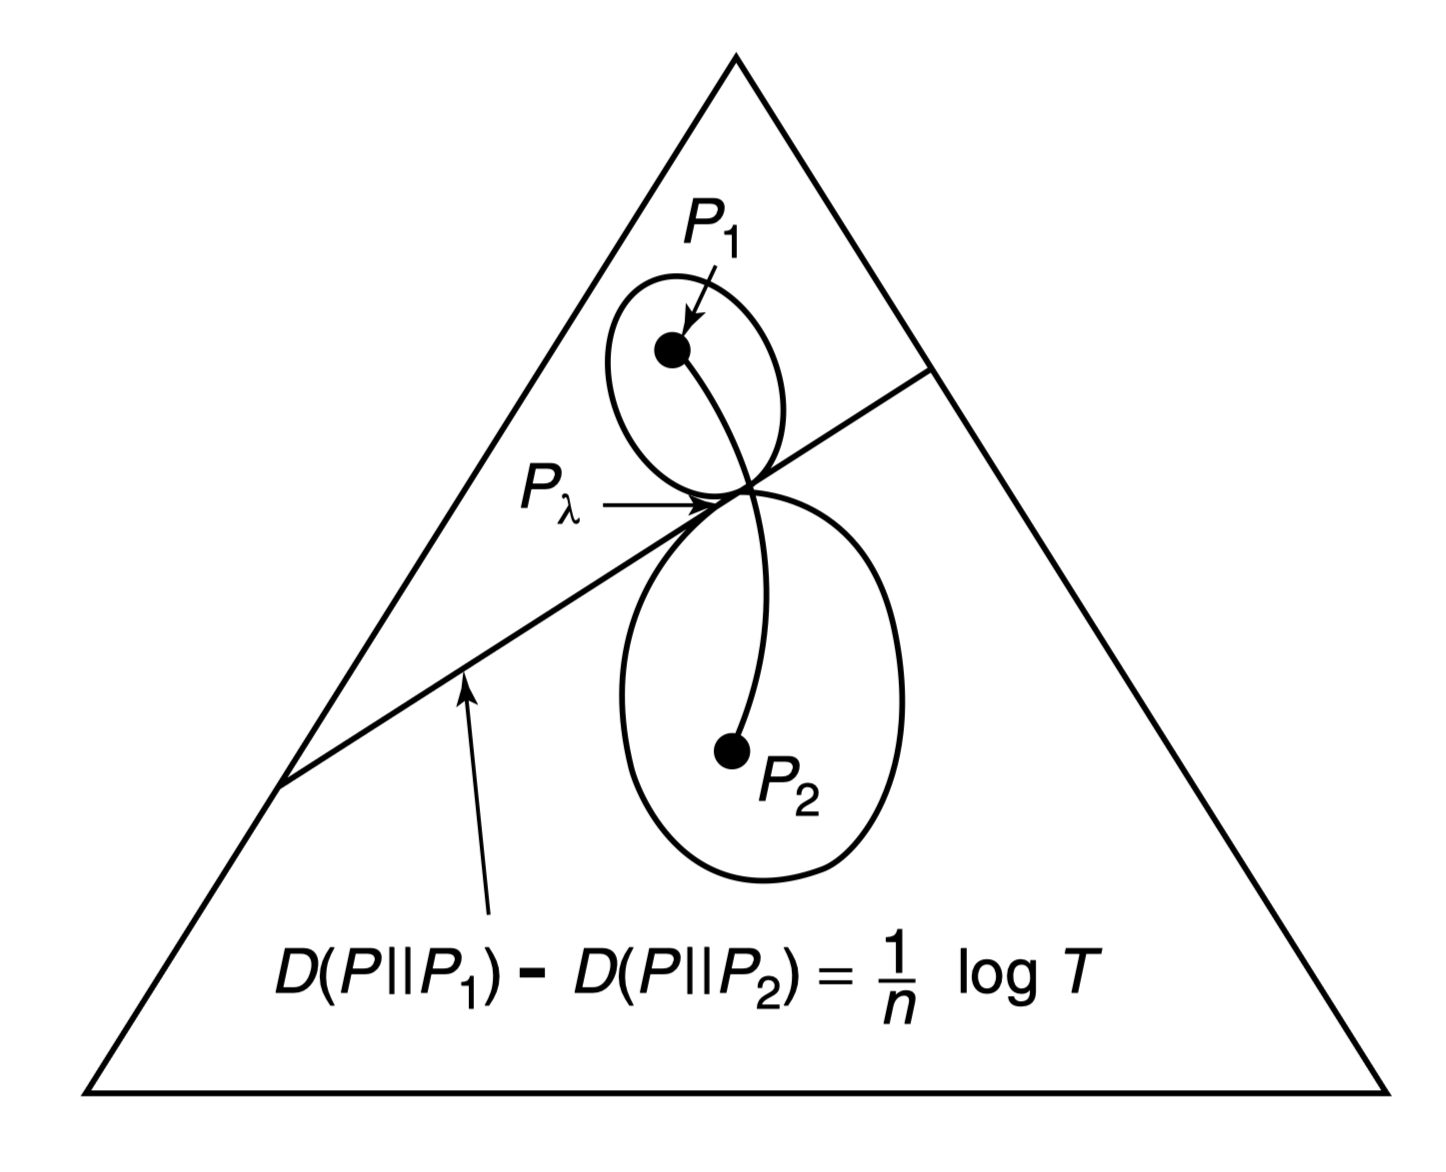
\includegraphics[width=0.5\linewidth]{Figs/fig6.png}
\centering
\caption{Likelihood ratio test on the probability simplex.}
		\label{ht:fig1}
\end{figure}

\subsubsection{Exponent in the Error Probabilities $\alpha$ and $\beta$}\label{ht:sssect2_1}
We now offer some informal arguments based on \cref{ld:thm1} to show how the two probabilities of error change with $n$ if using likelihood ratio test. Let $A$ denote the set on which $H_1$ is accepted. 
\begin{align*}
\alpha_{n}=P_{1}^{n}\left(P_{X^{n}} \in A\setcomp\right)
\end{align*}
Since the set $A\setcomp$ is closed, we can use \cref{ld:thm1} to show that the probability of error is determined essentially by the relative entropy of the closest member of $A\setcomp$ to $P_{1}$. Therefore,
\begin{align*}
\alpha_{n} \doteq 2^{-n D\left(P_{1}^{*}|| P_{1}\right)}
\end{align*}
where $P_{1}^{*}$ is the closest element of $B^{c}$ to distribution $P_{1} .$ Similarly,
\begin{align*}
\beta_{n} \doteq 2^{-n D\left(P_{2}^{*}|| P_{2}\right)}
\end{align*}
where $P_{2}^{*}$ is the closest element in $A$ to the distribution $P_{2}$. 

\tb{We next show $P_{1}^{*}=P_{2}^{*}$:}

Now minimizing $D\left(P \| P_{2}\right)$ subject to the constraint $D\left(P \| P_{2}\right)-$ $D\left(P \| P_{1}\right) \geq \frac{1}{n} \log T$ will yield the type in $A$ that is closest to $P_{2} .$ Setting up the minimization of $D\left(P \| P_{2}\right)$ subject to $D\left(P \| P_{2}\right)-D\left(P \| P_{1}\right)=$ $\frac{1}{n} \log T$ using Lagrange multipliers, we have
\begin{align*}
J(P)=\sum P(x) \log \frac{P(x)}{P_{2}(x)}+\lambda \sum P(x) \log \frac{P_{1}(x)}{P_{2}(x)}+\nu \sum P(x)
\end{align*}
Differentiating with respect to $P(x)$ and setting to 0, we have
\begin{align*}
\log \frac{P(x)}{P_{2}(x)}+1+\lambda \log \frac{P_{1}(x)}{P_{2}(x)}+v=0
\end{align*}

Solving this set of equations, we obtain the minimizing $P$ of the form
\begin{align}
P_{2}^{*}=P_{\lambda^{*}}=\frac{P_{1}^{\lambda}(x) P_{2}^{1-\lambda}(x)}{\sum_{a \in X } P_{1}^{\lambda}(a) P_{2}^{1-\lambda}(a)} \label{ht:eq3}
\end{align}
where $\lambda$ is chosen so that $D\left(P_{\lambda^{*}} \| P_{1}\right)-D\left(P_{\lambda^{*}} \| P_{2}\right)=\frac{1}{n} \log T$.
From the symmetry of expression \cref{ht:eq3}, it is clear that $P_{1}^{*}=P_{2}^{*}$ and that the probabilities of error behave exponentially with exponents given by the relative entropies $D\left(P^{*}|| P_{1}\right)$ and $D\left(P^{*}|| P_{2}\right)$. Also note from the equation that as $\lambda \rightarrow 1, P_{\lambda} \rightarrow P_{1}$ and as $\lambda \rightarrow 0, P_{\lambda} \rightarrow P_{2}$. The curve
that $P_{\lambda}$ traces out as $\lambda$ varies is a geodesic in the simplex. 
\begin{rema}{\bfs{explanation of above discussion}} \label{ht:rate}
We have shown that for likelihood ratio test, the $P_{1}^{*}=P_{2}^{*} = P^{*} $, where $P_{1}^{*}$ is the closest element of $A\setcomp$ to distribution $P_{1}$ and $P_{2}^{*}$ is the closest element in $A$ to the distribution $P_{2}$. We also get:
\begin{align}
\alpha_{n} \doteq 2^{-n D\left(P^{*}|| P_{1}\right)} \text{ and } \beta_{n} \doteq 2^{-n D\left(P^{*}|| P_{2}\right)} \label{ht:eqerr_rate}
\end{align}
We need to note here $P^{*}$ depends on the $T$ in the test \cref{ht:eqlrt} and the two exponents, $ D\left(P^{*}|| P_{1}\right)$ and  $D\left(P^{*}|| P_{2}\right)$, are different in general. We know $\lambda\to 1$ monotonically as  $T\to \infty$. Since $D\left(P_{\lambda} \| P_{1}\right)$ increases with $\lambda$ and $D\left(P_{\lambda} \| P_{2}\right)$ decreases with $\lambda$ (because if $T$ increases, the decision region $A$ is increases), the maximum value of the minimum of $\left\{D\left(P_{\lambda} \| P_{1}\right), D\left(P_{\lambda} \| P_{2}\right)\right\}$ is attained when they are equal.
If we care about the total error probabilities (putting into a Bayesian setting), since the one with small exponent will be the dominant one, we have that if $\lambda$ (and correspondingly $T$) is select such that $ D\left(P^{*}|| P_{1}\right)=D\left(P^{*}|| P_{2}\right)$, this is the best error exponent. More discussions are given in \cref{ht:ssec4}.

\end{rema}



\subsection{Neyman-Pearson Hypothesis Testing and Chernoff-Stein Lemma}\label{ht:ssec3}

We consider hypothesis testing in the case when one of the probabilities of error is held fixed and the other is made as small as possible. We will show that the other probability of error is exponentially small, with an exponential rate equal to the relative entropy between the two distributions. 

The method of proof uses a relative entropy version of the AEP:

\begin{thma}{\bfs{AEP for Relative Entropy}}
 Let $X_{1}, X_{2}, \ldots, X_{n}$ be a sequence of random variables drawn i.i.d. according to $P_{1}(x)$, and let $P_{2}(x)$ be any other distribution on $X$. Then
 \begin{align*}
     \frac{1}{n} \log \frac{P_{1}\left(X_{1}, X_{2}, \ldots, X_{n}\right)}{P_{2}\left(X_{1}, X_{2}, \ldots, X_{n}\right)} \rightarrow D\left(P_{1} \| P_{2}\right) \quad \text{in probability}.
 \end{align*}

\end{thma}
\begin{proof}
This follows directly from the weak law of large numbers.
\begin{align*}
\frac{1}{n} \log \frac{P_{1}\left(X_{1}, X_{2}, \ldots, X_{n}\right)}{P_{2}\left(X_{1}, X_{2}, \ldots, X_{n}\right)}&=\frac{1}{n} \log \frac{\prod_{i=1}^{n} P_{1}\left(X_{i}\right)}{\prod_{i=1}^{n} P_{2}\left(X_{i}\right)}\\
&=\frac{1}{n} \sum_{i=1}^{n} \log \frac{P_{1}\left(X_{i}\right)}{P_{2}\left(X_{i}\right)} \\
&\rightarrow E_{P_{1}} \log \frac{P_{1}(X)}{P_{2}(X)} \text { in probability } \\
&=D\left(P_{1}|| P_{2}\right)
\end{align*}
\end{proof}


Just as for the regular AEP, we can define a relative entropy typical sequence as one for which the empirical relative entropy is close to its expected value.

\begin{defa}{\bfs{Relative Entropy Typical Set $A_{\epsilon}^{(n)}\left(P_{1} \| P_{2}\right)$}}
Given $n$ and $\epsilon>0$, we define the relative entropy typical set as the sequence in $\calX^n$ whose ($\log$ average) likelihood ratio using measure $P_1$ and $P_2$ is close to the relative entropy of $P_1$ and $P_2$:
$$
A_{\epsilon}^{(n)}\left(P_{1} \| P_{2}\right) = \left\{\bx\in \calX^n\mid D\left(P_{1}|| P_{2}\right)-\epsilon \leq \frac{1}{n} \log \frac{P_{1}\left(x_{1}, x_{2}, \ldots, x_{n}\right)}{P_{2}\left(x_{1}, x_{2}, \ldots, x_{n}\right)} \leq D\left(P_{1}|| P_{2}\right)+\epsilon\right\}
$$
\end{defa} 

As a consequence of the relative entropy AEP, we can show that the relative entropy typical set satisfies the following properties:
\begin{thma}{\bfs{Properties of Relative Entropy Typical Set}}\label{ht:Properties}
\begin{enumerate}
    \item For $\bx\in A_{\epsilon}^{(n)}\left(P_{1} \| P_{2}\right)$, we have
    \begin{align*}
        P_{1}&\left(x_{1}, x_{2}, \ldots, x_{n}\right) 2^{-n\left(D\left(P_{1} \| P_{2}\right)+\epsilon\right)} \\
&\leq P_{2}\left(x_{1}, x_{2}, \ldots, x_{n}\right) \\
&\leq P_{1}\left(x_{1}, x_{2}, \ldots, x_{n}\right) 2^{-n\left(D\left(P_{1}|| P_{2}\right)-\epsilon\right)}
    \end{align*}
    \item $P_{1}\left(A_{\epsilon}^{(n)}\left(P_{1} \| P_{2}\right)\right)>1-\epsilon$, for $n$ sufficiently large.
    \item $P_{2}\left(A_{\epsilon}^{(n)}\left(P_{1}|| P_{2}\right)\right)<2^{-n\left(D\left(P_{1}|| P_{2}\right)-\epsilon\right)}$
    \item $P_{2}\left(A_{\epsilon}^{(n)}\left(P_{1}|| P_{2}\right)\right)>(1-\epsilon) 2^{-n\left(D\left(P_{1}|| P_{2}\right)+\epsilon\right)}$, for $n$ sufficiently large.
\end{enumerate}
\end{thma}

\begin{proof}
        We only need to show 3. and 4. since the other two conclusions are obvious.
\begin{align*}
  P_{2}&\left(A_{\epsilon}^{(n)}\left(P_{1} \| P_{2}\right)\right)=\sum_{x^{n} \in A_{\epsilon}^{(n)}\left(P_{1} \| P_{2}\right)} P_{2}\left(x_{1}, x_{2}, \ldots, x_{n}\right) \\
&\leq \sum_{x^{n} \in A_{\epsilon}^{(n)}\left(P_{1} \| P_{2}\right)} P_{1}\left(x_{1}, x_{2}, \ldots, x_{n}\right) 2^{-n\left(D\left(P_{1} \| P_{2}\right)-\epsilon\right)} \\
&=2^{-n\left(D\left(P_{1} \| P_{2}\right)-\epsilon\right)} \sum_{x^{n} \in A_{\epsilon}^{(n)}\left(P_{1}|| P_{2}\right)} P_{1}\left(x_{1}, x_{2}, \ldots, x_{n}\right) \\
&=2^{-n\left(D\left(P_{1} \| P_{2}\right)-\epsilon\right)} P_{1}\left(A_{\epsilon}^{(n)}\left(P_{1} \| P_{2}\right)\right) \\
&\leq 2^{-n\left(D\left(P_{1} \| P_{2}\right)-\epsilon\right)}  
\end{align*}
\begin{align*}
P_{2}&\left(A_{\epsilon}^{(n)}\left(P_{1} \| P_{2}\right)\right)=\sum_{x^{n} \in A_{\epsilon}^{(n)}\left(P_{1} \| P_{2}\right)} P_{2}\left(x_{1}, x_{2}, \ldots, x_{n}\right) \\
&\geq \sum_{x^{n} \in A_{\epsilon}^{(n)}\left(P_{1} \| P_{2}\right)} P_{1}\left(x_{1}, x_{2}, \ldots, x_{n}\right) 2^{-n\left(D\left(P_{1} \| P_{2}\right)+\epsilon\right)} \\
&=2^{-n\left(D\left(P_{1} \| P_{2}\right)+\epsilon\right)} \sum_{x^{n} \in A_{\epsilon}^{(n)}\left(P_{1} \| P_{2}\right)} P_{1}\left(x_{1}, x_{2}, \ldots, x_{n}\right) \\
&=2^{-n\left(D\left(P_{1} \| P_{2}\right)+\epsilon\right)} P_{1}\left(A_{\epsilon}^{(n)}\left(P_{1} \| P_{2}\right)\right) \\
&\geq(1-\epsilon) 2^{-n\left(D\left(P_{1} \| P_{2}\right)+\epsilon\right.},
\end{align*}
\end{proof}

\begin{rema}{\bfs{classical AEP typical set $A_{\epsilon}^{(n)}$ vs. relative entropy typical set $A_{\epsilon}^{(n)}\left(P_{1} \| P_{2}\right)$}}
\begin{enumerate}
    \item  Recall that in the classical AEP typical set $A_{\epsilon}^{(n)}$ for $H(X)$ we only have one probability distribution, say $P_1$. The classical AEP typical set $A_{\epsilon}^{(n)}$ can be regarded as a special case for relative entropy typical set $A_{\epsilon}^{(n)}\left(P_{1} \| P_{2}\right)$ with $P_{2}$ being the uniform measure. 
    \item 
 We know classical $A_{\epsilon}^{(n)}$ has the property of containing $\geq 1-\epsilon$ of the probability mass w.r.t to $P_1$. It was showed that $A_{\epsilon}^{(n)}$ has $\geq (1-\epsilon)2^{n(H(X)+\epsilon)}$ (i.e. $\doteq$ $2^{n(H(X)}$) elements , and for any other set $B_{n}$ with this property it must has size equals $A_{\epsilon}^{(n)}$ \tb{to first order in exponent}. Note that the size of a set can be regarded as the probability mass w.r.t to uniform measure (times $|\calX|^{n}$). \label{ht:reit2}
 
 \item In the context of relative entropy typical set $A_{\epsilon}^{(n)}\left(P_{1} \| P_{2}\right)$, the analogy question will be: if $B_{n}$ has the property of containing $\geq 1-\epsilon$ of the probability mass w.r.t to $P_1$ (i.e. 2. in \cref{ht:Properties}),  can we find a $B_{n}$ with less probability, w.r.t $P_2$, than $2^{-nD(P_{1} \| P_{2})}$ (from 3. and 4. in \cref{ht:Properties}). Note we have already know  if $P_2$ is the uniform measure, from above, the answer is ``no'' and they must have the probability w.r.t  $P_2$ with the same exponent. The general answer is still ``no'' proved by the following \cref{ht:lem1}. 
\end{enumerate}
\end{rema}

\begin{lema}{\bfs{The Smaller Property of Typical Set}} \label{ht:lem1}
Let $B_{n} \subseteq \mathcal{X}^{n}$ be any set of sequences $x_{1}, x_{2}, \ldots, x_{n}$ such that $P_{1}\left(B_{n}\right)>1-\epsilon$. Let $P_{2}$ be any other distribution such that $D\left(P_{1}|| P_{2}\right)$ $<\infty$. Then 
\begin{align*}
    P_{2}\left(B_{n}\right)>(1-2 \epsilon) 2^{-n\left(D\left(P_{1} \| P_{2}\right)+\epsilon\right)}
\end{align*}
\end{lema} 
\begin{proof}
For simplicity, we will denote $A_{\epsilon}^{(n)}\left(P_{1} \| P_{2}\right)$ by $A_{n}$. Since $P_{1}\left(B_{n}\right)$ $>1-\epsilon$ and $P\left(A_{n}\right)>1-\epsilon$, we have, by the union of events bound, $P_{1}\left(A_{n}^{c} \cup B_{n}^{c}\right)<2 \epsilon$, or equivalently, $P_{1}\left(A_{n} \cap B_{n}\right)>1-2 \epsilon$. Thus,
\begin{align*}
P_{2}&\left(B_{n}\right) \geq P_{2}\left(A_{n} \cap B_{n}\right)\\
&=\sum_{x^{n} \in A_{n} \cap B_{n}} P_{2}\left(x^{n}\right) \\
& \geq \sum_{x^{n} \in A_{n} \cap B_{n}} P_{1}\left(x^{n}\right) 2^{-n\left(D\left(P_{1} \| P_{2}\right)+\epsilon\right)} \\
&=2^{-n\left(D\left(P_{1} \| P_{2}\right)+\epsilon\right)} \sum_{x^{n} \in A_{n} \cap B_{n} }P_{1}\left(x^{n}\right) \\
&=2^{-n\left(D\left(P_{1} \| P_{2}\right)+\epsilon\right)} P_{1}\left(A_{n} \cap B_{n}\right) \\
& \geq 2^{-n\left(D\left(P_{1} \| P_{2}\right)+\epsilon\right)}(1-2 \epsilon),
\end{align*}
\end{proof} 

We now can prove the relative entropy is the best exponent in probability of error in Neyman-Pearson Hypothesis Testing setting as the following \cref{ht:Chernoff-Stein}.

\begin{thma}{\bfs{Chernoff-Stein Lemma}}\label{ht:Chernoff-Stein}
Let $X_{1}, X_{2}, \ldots, X_{n}$ be
i.i.d. $\sim Q .$ Consider the hypothesis test between two alternatives, $Q=P_{1}$ and $Q=P_{2}$, where $D\left(P_{1} \| P_{2}\right)<\infty$. Let $A_{n} \subseteq \mathcal{X}^{n}$ be an acceptance region for hypothesis $H_{1} .$ Let the probabilities of error be
$$
\alpha_{n}=P_{1}^{n}\left(A_{n}^{c}\right), \quad \beta_{n}=P_{2}^{n}\left(A_{n}\right)
$$
and for any $0<\epsilon<\frac{1}{2}$, define
$$
\beta_{n}^{\epsilon}=\min _{
\begin{array}{c}
A_{n} \subseteq \mathcal{X}^{n} \\
\alpha_{n}<\epsilon
\end{array}
} \beta_{n}
$$
Then
$$
\lim _{n \rightarrow \infty} \frac{1}{n} \log \beta_{n}^{\epsilon}=-D\left(P_{1}|| P_{2}\right)
$$
\end{thma} 
\begin{proof}
We prove this theorem in two parts:\\
1.  Achievability: In the first part we exhibit a sequence of sets $A_{n}$ for which the probability of error $\beta_{n}$ goes exponentially to zero as with exponent $D\left(P_{1} \| P_{2}\right) .$ \\
2. Converse: In the second part we show that no other sequence of sets can have a lower exponent in the probability of error. 

For the first part, we choose as the sets $A_{n}=A_{\epsilon}^{(n)}\left(P_{1} \| P_{2}\right) .$ As proved in Property 2. of \cref{ht:Properties}, this sequence of sets has $P_{1}\left(A_{n}^{c}\right)<\epsilon$ for $n$ large enough. Also,
$$
\lim _{n \rightarrow \infty} \frac{1}{n} \log P_{2}\left(A_{n}\right) \leq-\left(D\left(P_{1} \| P_{2}\right)-\epsilon\right)
$$
from Property 3. of \cref{ht:Properties}. Thus, the relative entropy typical set satisfies all the requirements.

To show that no other sequence of sets can to better, consider any sequence of sets $B_{n}$ with $P_{1}\left(B_{n}\right)>1-\epsilon$. By \cref{ht:lem1}, we have $P_{2}\left(B_{n}\right)>(1-2 \epsilon) 2^{-n\left(D\left(P_{1}|| P_{2}\right)+\epsilon\right)}$, and therefore
$$
\begin{aligned}
\lim _{n \rightarrow \infty} \frac{1}{n} & \log P_{2}\left(B_{n}\right)>-\left(D\left(P_{1}|| P_{2}\right)+\epsilon\right)+\lim _{n \rightarrow \infty} \frac{1}{n} \log (1-2 \epsilon) \\
\quad=&-\left(D\left(P_{1} \| P_{2}\right)+\epsilon\right)
\end{aligned}
$$
Thus, no other sequence of sets has a probability of error exponent better than $D\left(P_{1} \| P_{2}\right)$. Thus, the set sequence $A_{n}=A_{\epsilon}^{(n)}\left(P_{1}|| P_{2}\right)$ is asymptotically optimal in terms of the exponent in the probability. $\square$
\end{proof}

\begin{rema}{\bfs{asymptotic optimal vs. optimal}}
The relative entropy typical set is only optimal in the sense of asymptotic and is not the optimal set for any fixed hypothesis-testing problem. The optimal set that minimizes the probabilities of error is that given by the Neyman-Pearson lemma.
\end{rema}


\subsection{Bayesian Hypothesis Testing and Chernoff Information}\label{ht:ssec4}

In this section, we consider Bayesian hypothesis testing setting in which we assign prior probabilities to both hypotheses. Specifically we consider the \tb{minimum probability-of-error ($\P(e)$) criterion} with the cost setting $C_{ii}= 0$ and $C_{ij}= 1$ for $i\ne j$. Some of the the results are already shown in the discussion in\cref{ht:sssect2_1}. From \cref{ht:eq1}, we know the overall probability of error is
    \begin{align}
        P_{e}^{(n)} &=  \P(\bH = H_1)P_{1}^{n}\left(A\setcomp\right) + \P(\bH = H_2)P_{2}^{n}\left(A\right)\nn
         &= \P(\bH = H_1)\alpha_n + \P(\bH = H_2)\beta_n
    \end{align}
Asymptotically, only the exponent of the $\alpha_n$ and $\beta_n$ will affects the exponent of $P_{e}^n$. Let 
\begin{align*}
D^{*}=\lim _{n \rightarrow \infty}-\frac{1}{n} \log \min _{A_{n} \subseteq \calX ^{n}} P_{e}^{(n)}
\end{align*}
\subsubsection{Achievability and Converse of Chernoff Information Bound}
\begin{thma}{\bfs{Chernoff}}\label{ht:thm_chrenoff_rate}
The best achievable exponent in the Bayesian probability of error is $D^{*}$, where
\begin{align*}
D^{*}=D\left(P_{\lambda^{*}} \| P_{1}\right)=D\left(P_{\lambda^{*}} \| P_{2}\right)
\end{align*}
with
\begin{align*}
P_{\lambda}=\frac{P_{1}^{\lambda}(x) P_{2}^{1-\lambda}(x)}{\sum_{a \in X } P_{1}^{\lambda}(a) P_{2}^{1-\lambda}(a)}
\end{align*}
and $\lambda^{*}$ the value of $\lambda$ such that
\begin{align*}
D\left(P_{\lambda^{*}} \| P_{1}\right)=D\left(P_{\lambda^{*}} \| P_{2}\right)
\end{align*}
\end{thma} 
\begin{rema}{\bfs{Additional Discussion for \cref{ht:thm_chrenoff_rate}}}
We have proved using likelihood ratio test, we can get the best exponent is $D^{*}$. This is the ``achievability'' aspect. However in \cref{ht:thm_chrenoff_rate} we already state that this is the best exponent with the ``converse'' aspect. This is because from \cref{ht:thm1} we know likelihood ratio test is optimal under Bayesian hypothesis testing. In addtion, we give a new proof of the  ``converse'' part in \cref{ht:sssec_cib} using MAP which is the optimal decision rule under \tb{minimum probability-of-error criterion}.
\end{rema}
\begin{proof}
Using likelihood ratio test, from \cref{ht:eq3,ht:eqerr_rate}, we know \begin{align}
\alpha_{n} \doteq 2^{-n D\left(P_{\lambda}|| P_{1}\right)} \text{ and } \beta_{n} \doteq 2^{-n D\left(P_{\lambda}|| P_{2}\right)} 
\end{align}
and 
\begin{align*}
P_{e} \doteq 2^{-n \min \left\{D\left(P_{\lambda} \| P_{1}\right), D\left(P_{\lambda} \| P_{2}\right)\right\}}
\end{align*}
since the exponential rate is determined by the worst exponent. From the discussion in \cref{ht:rema1}, the maximum value of the minimum of $\left\{D\left(P_{\lambda} \| P_{1}\right), D\left(P_{\lambda} \| P_{2}\right)\right\}$ is attained when they are equal.  Hence, we choose $\lambda$ so that
\begin{align*}
D\left(P_{\lambda} \| P_{1}\right)=D\left(P_{\lambda} \| P_{2}\right)
\end{align*}
\end{proof}

\begin{defa}{\bfs{Chernoff Information I }} As shown in \cref{ht:thm_chrenoff_rate}, we call the best achievable error exponent $D^{*}$ under Bayesian hypothesis testing as Chernoff Information $C\left(P_{1}, P_{2}\right)$, where
\begin{align}
C\left(P_{1}, P_{2}\right)\coloneqq D^{*}=D\left(P_{\lambda^{*}} \| P_{1}\right)=D\left(P_{\lambda^{*}} \| P_{2}\right)\label{ht:eqI}
\end{align}
\end{defa}
Another equivalent definition of Chernoff information is 
\begin{defa}{\bfs{Chernoff Information II}} 
\begin{align}
C\left(P_{1}, P_{2}\right)\coloneqq -\min _{0 \leq \lambda \leq 1} \log \left(\sum_{x} P_{1}^{\lambda}(x) P_{2}^{1-\lambda}(x)\right)\label{ht:eqII}
\end{align}
\end{defa}

The equivalence of \cref{ht:eqI,ht:eqII} can be shown by take derivative w.r.t. $\lambda$ in  \cref{ht:eqII}.


\subsubsection{Another Proof for Converse of Chernoff Information Bound}\label{ht:sssec_cib}

We next display the usual derivation of the converse of Chernoff information bound with  \cref{ht:eqII} formula:
\begin{align*}
    \text{There is no better achievable error exponent than Chernoff information } C\left(P_{1}, P_{2}\right).
\end{align*}


As we have introduced in \cref{ht:rema1}, the maximum a posteriori probability decision rule minimizes the Bayesian probability of error:
\begin{align}
    A=\left\{ \bx : \frac{\P(\bH = H_1) P^n_{1}( \bx )}{\P(\bH = H_2) P^n_{2}( \bx )}>1\right\}\label{ht:eqmap}
\end{align}
and the probability of error for this rule therefore is

    \begin{align}
        P_{e}^{(n)} &=  \P(\bH = H_1)P_{1}^{n}\left(A\setcomp\right) + \P(\bH = H_2)P_{2}^{n}\left(A\right)\nn
        &=\sum_{\bx\in\calX^n} \min \left\{\P(\bH = H_1) P^n_{1}, \P(\bH = H_2) P^n_{2}\right\}
    \end{align}
For any two positive numbers $a$ and $b$, we have
\begin{align*}
\min \{a, b\} \leq a^{\lambda} b^{1-\lambda} \quad \text { for all } 0 \leq \lambda \leq 1
\end{align*}

Using this to continue the chain, we have
\begin{align*}
\begin{aligned}
P_{e}^{(n)}  &=\sum_{\bx\in\calX^n} \min \left\{\P(\bH = H_1)  P^n_{1}, \P(\bH = H_2)  P^n_{2}\right\} \\
& \leq \sum_{\bx\in\calX^n}\left(\P(\bH = H_1)  P^n_{1}\right)^{\lambda}\left(\P(\bH = H_2)  P^n_{2}\right)^{1-\lambda} \\
& \leq \sum_{\bx\in\calX^n} (P^n_{1})^{\lambda} (P^n_{2})^{1-\lambda}\nn
& = \sum_{\bx\in\calX^n} \prod_{i=1}^{n} (P_{1}(x_i))^{\lambda}
(P_{2}(x_i))^{1-\lambda}\nn
& =  \prod_{i=1}^{n} \sum_{x_i\in\calX} (P_{1}(x_i))^{\lambda}
(P_{2}(x_i))^{1-\lambda}\nn
\end{aligned}
\end{align*}
Hence, we have
\begin{align*}
\frac{1}{n} \log P_{e}^{(n)} \leq \log \sum_{x\in\calX} P_{1}^{\lambda}(x) P_{2}^{1-\lambda}(x)
\end{align*}
Since this is true for all $\lambda$, we can take the minimum over $0 \leq \lambda \leq 1$, resulting in the Chernoff information bound. This proves that the exponent is no better than $C\left(P_{1}, P_{2}\right)$. 
\begin{rema}{\bfs{negligibility of the \emph{a priori} probability}}
Note that the Bayesian error exponent does not depend on the actual value of $\P(\bH = H_1) $ and $\P(\bH = H_2) $, as long as they are nonzero. Essentially, the effect of the prior is washed out for large sample sizes. From \cref{ht:eqmap}, after taking the $\log$ and dividing by $n$, the MAP test can be rewritten as
$$
\frac{1}{n} \log \frac{\P(\bH = H_1) }{\P(\bH = H_2) }+\frac{1}{n} \sum_{i} \log \frac{P_{1}\left(X_{i}\right)}{P_{2}\left(X_{i}\right)}>0
$$
where the second term tends to $D\left(P_{1} \| P_{2}\right)$ or $-D\left(P_{2}|| P_{1}\right)$ accordingly as $P_{1}$ or $P_{2}$ is the true distribution. The first term tends to 0 , and the effect of the prior distribution washes out.
\end{rema}

\section{Estimation, Fisher Information and the Cram\'{e}r Inequality}
In this section we study \tb{nonrandom} parameter estimation. 

\begin{defa}{\bfs{Parameter Set $\Theta$ and Observation Density}}
Let $\{f(x ; \theta)\}, \theta \in \Theta$, denote an indexed family of densities, $f(x ; \theta) \geq 0, \int f(x ; \theta) d x=1$ for all $\theta \in \Theta$. Here $\Theta$ is called the parameter set.
\end{defa}definitions. 

\begin{defa}{\bfs{Estimator}}
An estimator for $\theta$ for sample size $n$ is a function $T: \calX^{n} \rightarrow \Theta$. $T$ is therefore a random variable
\end{defa} 

\begin{defa}{\bfs{Error}}
We will call the difference $$e_T(X^n) = T(X^n)-\theta$$ the error of the estimator $T$. The error is a random variable since $T$ is a random variable.
\end{defa} 

\begin{defa}{\bfs{Bias and Unbiased Estimator}}
The bias $b_T(X^n)$ of an estimator $T\left(X_{1}, X_{2}, \ldots, X_{n}\right)$ for the parameter $\theta$ is the expected value of the error of the estimator:
$$b_T(X^n)=\E{\theta} T\left(X_{1}, X_{2}, \ldots, X_{n}\right)-\theta.$$

 $\E_{\theta}$ means the expectation is taken w.r.t. $f(x ; \theta)$. The estimator is said to be unbiased if the bias is zero \tb{for all} $\theta \in \Theta$ (i.e., the expected value of the estimator is equal to the parameter).
\end{defa} 


The bias is the expected value of the error, and the fact that it is zero does not guarantee that the error is low with high probability. We often qualify the estimator using \tb{mean-square estimation error}:
$$\E{\theta}[[e_T(X^n)]^2] = \E{\theta}[\left(T_{1}\left(X_{1}, X_{2}, \ldots, X_{n}\right)-\theta\right)^{2}]$$

One desirable \tb{asymptotic} property is \tb{consistent}:

\begin{defa}{\bfs{Consistent in $\calL_2$ Convergence}}
An estimator $T\left(X_{1}, X_{2}, \ldots, X_{n}\right)$ for $\theta$ is said to be consistent in $\calL_2$ convergence if $T\left(X_{1}, X_{2}, \ldots, X_{n}\right) \rightarrow \theta$ in $\calL_2$ as $n \rightarrow \infty$
\end{defa}

\begin{defa}{\bfs{Consistent in Probability}}
An estimator $T\left(X_{1}, X_{2}, \ldots, X_{n}\right)$ for $\theta$ is said to be consistent in probability if $T\left(X_{1}, X_{2}, \ldots, X_{n}\right) \rightarrow \theta$ in probability as $n \rightarrow \infty$
\end{defa}

We can also  rank estimators on the basis of their mean-squared error for finite samples using the concept of dominant:

\begin{defa}{\bfs{Dominate}}
An estimator $T_{1}\left(X_{1}, X_{2}, \ldots, X_{n}\right)$ is said to dominate another estimator $T_{2}\left(X_{1}, X_{2}, \ldots, X_{n}\right)$ if, \tb{for all} $\theta$,
$$
\E{\theta}\left(T_{1}\left(X_{1}, X_{2}, \ldots, X_{n}\right)-\theta\right)^{2} \leq \E{\theta}\left(T_{2}\left(X_{1}, X_{2}, \ldots, X_{n}\right)-\theta\right)^{2}
$$
\end{defa}
This raises a natural question: Is there a best estimator of $\theta$ that dominates every other estimator? To answer this question, we derive the Cram\'{e}r-Rao lower bound on \tb{the mean-squared error of any estimator} in \cref{es:remaboundany}. We first define the score function of the distribution $f(x ; \theta) .$ We then use the Cauchy-Schwarz inequality to prove the Cramér-Rao lower bound on the \tb{variance} of all \tb{unbiased} estimators in \cref{es:thm1}.

Before we begin, we show the relation between the variance of estimators and the mean-square estimation error.
\begin{rema}{\bfs{estimation variance and mean-square error}}

\tb{error variance $\operatorname{var}(e_T) =$ estimator variance $\operatorname{var}(T)$}:
$$
\operatorname{var}(e_T)=\E{\theta}\left[\left[e_T(X)-b_T(X)\right]^2\right]=\E{\theta}\left[\left[T(X)-\E{\theta}T(X)\right]^2\right] = \operatorname{var}(T)
$$
\tb{mean-square estimation error $=$ error variance $\operatorname{var}(e_T)+$ square of bias $b_T^2$}:
$$\operatorname{var}(e_T)=\E{\theta}[[e_T(X^n)]^2]-b_T^2\Longrightarrow \E{\theta}[[e_T(X^n)]^2] = \operatorname{var}(e_T)+b_T^2$$

We therefore have that if we restrict our self to the class of \tb{unbiased} estimators, to minimize the mean-square estimation error is to minimize the error variance (i.e. estimator variance). And \cref{es:thm1} shows the mean-square estimation error bound in such a scenario.
\end{rema}

\begin{rema}{\bfs{$\theta$ with high dimensions (multiparameter)}}
I would like to mention a little bit for the high dimension case, where variance is replaced by the covariance. The  mean-square estimation error is estimate by the $\calL_2$ error and equals the trace of the error variance for unbiased  estimators. The Cram\'{e}r-Rao Inequality is then replaced by covariance matrix with positive semi-definite operator $\succeq$. More specifically, we can generalize the concept of Fisher information to the multiparameter case, in which case we define the Fisher information matrix $J(\theta)$ with elements
$$
J_{i j}(\theta)=\int f(x ; \theta) \frac{\partial}{\partial \theta_{i}} \ln f(x ; \theta) \frac{\partial}{\partial \theta_{j}} \ln f(x ; \theta) d x
$$
The Cramér-Rao inequality becomes the matrix inequality
$$
\Sigma \succeq J^{-1}(\theta)
$$
where $\Sigma$ is the covariance matrix of a set of unbiased estimators for the parameters $\theta$ and $\Sigma \succeq J^{-1}(\theta)$ in the sense that the difference $\Sigma-J^{-1}$ is a nonnegative definite matrix.

\end{rema}

\begin{defa}{\bfs{Score}} The score $V$ is a random variable defined by
$$
V(X)=\frac{\partial}{\partial \theta} \ln f(X ; \theta)=\frac{\frac{\partial}{\partial \theta} f(X ; \theta)}{f(X ; \theta)},
$$
where $X \sim f(x ; \theta)$.
\end{defa}
\begin{rema}{\bfs{mean value of the score}}
$$
\begin{aligned}
\E{\theta}V &=\int \frac{\frac{\partial}{\partial \theta} f(x ; \theta)}{f(x ; \theta)} f(x ; \theta) d x \\
&=\int \frac{\partial}{\partial \theta} f(x ; \theta) d x \\
&=\frac{\partial}{\partial \theta} \int f(x ; \theta) d x \\
&=\frac{\partial}{\partial \theta} 1 \\
&=0
\end{aligned}
$$

\end{rema}
 
We therefore have $$\E{\theta}V^{2}=\operatorname{var}(V).$$ The variance of the score has a special significance.
\begin{defa}{\bfs{Fisher Information}} The Fisher information $J_X(\theta)$ is the variance of the score:
$$
J_{X}(\theta)=\operatorname{var}(V)=\E_{\theta}\left[\frac{\partial}{\partial \theta} \ln f(X ; \theta)\right]^{2}
$$
Whenever it is clear from the context, we use abbreviation $J(\theta)$ without explicitly mentioning $X$.
\end{defa}

\begin{rema}{\bfs{Fisher information of $n$ \gls{iid} samples}}
If we consider a sample of $n$ random variables $X_{1}, X_{2}, \ldots, X_{n}$ drawn
i.i.d. $\sim f(x ; \theta)$, we have
$$
f\left(x_{1}, x_{2}, \ldots, x_{n} ; \theta\right)=\prod_{i=1}^{n} f\left(x_{i} ; \theta\right)
$$
and the score function is the sum of the individual score functions,
$$
\begin{aligned}
V\left(X_{1}, X_{2}, \ldots, X_{n}\right) &=\frac{\partial}{\partial \theta} \ln f\left(X_{1}, X_{2}, \ldots, X_{n} ; \theta\right) \\
&=\sum_{i=1}^{n} \frac{\partial}{\partial \theta} \ln f\left(X_{i} ; \theta\right) \\
&=\sum_{i=1}^{n} V\left(X_{i}\right)
\end{aligned}
$$
where the $V\left(X_{i}\right)$ are independent, identically distributed with zero mean. Hence, the $n$-sample Fisher information is
$$
\begin{aligned}
J_{n}(\theta) &=\E{\theta}\left[\frac{\partial}{\partial \theta} \ln f\left(X_{1}, X_{2}, \ldots, X_{n} ; \theta\right)\right]^{2} \\
&=\E{\theta} V^{2}\left(X_{1}, X_{2}, \ldots, X_{n}\right) \\
&=\E{\theta}\left(\sum_{i=1}^{n} V\left(X_{i}\right)\right)^{2} \\
&=\sum_{i=1}^{n} \E{\theta} V^{2}\left(X_{i}\right) \\
&=n J(\theta) .
\end{aligned}
$$
In other words, the Fisher information for $n$ i.i.d. samples is $n$ times the individual Fisher information. 
\end{rema}

\begin{thma}{\bfs{Cram\'{e}r-Rao Inequality}}\label{es:thm1}
The mean-squared error of any \tb{unbiased estimator} $T(X)$ of the parameter $\theta$ is lower bounded by the reciprocal of the Fisher information:
$$
\operatorname{var}(T) \geq \frac{1}{J_X(\theta)}
$$
\end{thma}

\begin{proof}
Let $V$ be the score function and $T$ be the estimator. By the Cauchy-Schwarz inequality, we have
$$
\left(\E{\theta}\left[\left(V-\E{\theta} V\right)\left(T-\E{\theta} T\right)\right]\right)^{2} \leq \E{\theta}\left(V-\E{\theta} V\right)^{2} \E{\theta}\left(T-\E{\theta} T\right)^{2}
$$
Since $T$ is unbiased, $\E{\theta} T=\theta$ for all $\theta .$ We also have proved $\E{\theta} V=0$ and hence $\E{\theta}\left(V-\E{\theta} V\right)\left(T-\E{\theta} T\right)=\E{\theta}(V T) .$ Also, by definition, $\operatorname{var}(V)=J(\theta)$
Substituting these conditions in (11.281), we have
$$
\left[\E{\theta}(V T)\right]^{2} \leq J(\theta) \operatorname{var}(T)
$$
Now,
\begin{align*}
   \E{\theta}(V T)&=\int \frac{\frac{\partial}{\partial \theta} f(x ; \theta)}{f(x ; \theta)} T(x) f(x ; \theta) \ud x\\
&=\int \frac{\partial}{\partial \theta} f(x ; \theta) T(x) d x \\
&=\frac{\partial}{\partial \theta} \int f(x ; \theta) T(x) d x \\
&=\frac{\partial}{\partial \theta} E_{\theta} T \\
&=\frac{\partial}{\partial \theta} \theta \\
&=1 
\end{align*}

where the interchange of differentiation and integration can be justified using the bounded convergence theorem for appropriately well behaved $f(x ; \theta)$. We therefore get
$$
\operatorname{var}(T) \geq \frac{1}{J(\theta)},
$$
which is the Cramér-Rao inequality for unbiased estimators.
\end{proof}
\begin{rema}{\bfs{Cram\'{e}r-Rao lower bound for arbitrary estimator}}\label{es:remaboundany}
By essentially the same arguments, we can show that for any estimator
$$
\E{\theta}(T-\theta)^{2} \geq \frac{\left(1+b_{T}^{\prime}(\theta)\right)^{2}}{J(\theta)}+b_{T}^{2}(\theta)
$$
where $b_{T}(\theta)=E_{\theta} T-\theta$ and $b_{T}^{\prime}(\theta)$ is the derivative of $b_{T}(\theta)$ with respect to $\theta$.
\end{rema}


\begin{defa}{\bfs{Efficient}}
An unbiased estimator $T$ is said to be efficient if it meets the Cramér-Rao bound with equality [i.e., if $\operatorname{var}(T)=\frac{1}{J(\theta)}$ ]
\end{defa} 



\blue{this section may need update}








\bibliographystyle{IEEEtran}
\bibliography{IEEEabrv,StringDefinitions,adv_dnn}
\end{document}
